% Dissertação do INF-UFG com texto em português formatado com LaTeX.
% A classe local preserva o modelo institucional e adiciona compatibilidade
% com o motor XeTeX usado pelo Tectonic.
\documentclass[dissertacao]{inf-ufg-tectonic}
\usepackage{amsmath}
% Opções da classe inf-ufg (ao usar mais de uma, separe por vírgulas)
%   [tese]         -> Tese de doutorado.
%   [dissertacao]  -> Dissertação de mestrado (padrão).
%   [monografia]   -> Monografia de especialização.
%   [relatorio]    -> Relatório final de graduação.
%   [abnt]         -> Usa o estilo "abnt-alf" de citação bibliográfica.
%   [nocolorlinks] -> Os links de navegação no texto ficam na cor preta.
%                     Use esta opção para gerar o arquivo para impressão
%                     da versão final do seu texto!!!

%----------------------------------------------------- INICIO DO DOCUMENTO %
\begin{document}
%\selectlanguage{portuguese}

%------------------------------------------ AUTOR, TÍTULO E DATA DE DEFESA %
\autor{ Pedro Henrique Sanches} % (José da Silva)
\autorR{ Sanches, Pedro Henrique} % (da Silva, José)

\titulo{IVF/SPEA2: Um algoritmo híbrido SPEA2 com Fertilização In Vitro para Otimização Multiobjetivo}
% \subtitulo{ Subtítulo do Trabalho}

\cidade{ Goiânia} % Nome da cidade em foi desenvolvido o trabalho
\dia{} % Definir somente após confirmação da data de defesa.
\mes{ 06} % Data da apresentação/defesa do trabalho
\ano{ 2025} % Formato numérico: \dia{01}, \mes{01} e \ano{2009}

%-------------------------------------------------------------- ORIENTADOR %
\orientador{ Celso Gonçalves Camilo Junior }
\orientadorR{ CAMILO-JUNIOR, CELSO}
% Use os comandos a seguir se for Orientadora e nao Orientador.
%\orientadora{ Nome da Orientadora}
%\orientadoraR{ Nome Reverso da Orientadora}

% \coorientador{ Nome do Co-orientador}
% \coorientadorR{ Nome Reverso do Co-orientador}
% Use os comandos a seguir se for Co-orientadora e nao Coorientador.
%\coorientadora{\textless Nome da Co-orientadora}
%\coorientadoraR{\textless Nome Reverso da Co-orientadora}

%-------------------------------------------------- INSTITUIÇÃO E PROGRAMA %
\universidade{ Universidade Federal de Goiás} % {Universidade Federal de Goiás}
\uni{ UFG }         % UFG
\unidade{ Instituto de Informática} %Instituto de Informática
% \departamento{ Nome do Departamento} %Unidades com mais de um depto.

\universidadeco{ Nome da Universidade do Co-orientador}
\unico{ Sigla da Universidade do Co-orientador}
\unidadeco{ Nome da Unidade Acadêmica do Co-orientador}

\programa{ Computação } % Computação
\concentracao{ Sistemas Inteligentes}

%-------------------------------------------------- ELEMENTOS PRÉ-TEXTUAIS %
\capa    % Gera o modelo da capa externa do trabalho
% A autorização depende da data definitiva de defesa.
% \publica % Gera a autorização para publicação em formato eletrônico
\rosto   % Primeira folha interna do trabalho

% A folha de aprovação permanece desativada até a confirmação da banca.
% \input{./pre/pre_aprovacao}
\direitos{Graduou-se em Ciência da Computação pela Universidade Federal de Goiás (UFG). Ingressou no mestrado pelo Programa de Pós-Graduação em Ciência da Computação (PPGCC) da UFG, com área de concentração em Sistemas Inteligentes. Mantém engajamento ativo na área de Inteligência Artificial, participando de grupos de estudo dedicados ao tema, e contribuiu em soluções desenvolvidas no âmbito do Centro de Excelência em Inteligência Artificial (CEIA) da UFG.}
% \input{./pre/pre_dedicatoria}
% \input{./pre/pre_agradecimentos}
% \input{./pre/pre_epigrafe}
\chaves{Fertilização, Vitro, IVF, Evolucionário, Evolutivo, SPEA2, Multi-Objetivo}

\begin{resumo} 
Problemas de Otimização Multiobjetivo (MOPs) frequentemente apresentam objetivos conflitantes e espaços de busca complexos, impondo desafios aos métodos de otimização tradicionais. O Algoritmo Evolucionário de Força Pareto 2 (SPEA2) é uma abordagem bem estabelecida para lidar com tais problemas, mas pode enfrentar limitações no balanceamento entre convergência e diversidade em cenários complexos. Este artigo propõe o IVF/SPEA2, um algoritmo híbrido que integra o método de Fertilização In Vitro (IVF) ao SPEA2 para aprimorar o desempenho por meio de manipulação genética direcionada. O IVF/SPEA2 foi avaliado utilizando quatro conjuntos de benchmarks amplamente reconhecidos ZDT, DTLZ, WFG e MaF cobrindo uma considerável gama de geometrias de fronteira de Pareto e complexidades de problemas. O desempenho foi medido utilizando a métrica de Distância Geracional Invertida (IGD), com a significância estatística avaliada por meio do teste de soma de postos de Wilcoxon em 100 execuções independentes. Os resultados demonstram que o IVF/SPEA2 alcança melhorias estatisticamente significativas em relação ao SPEA2 canônico em inúmeros problemas bi-objetivo e tri-objetivo, particularmente em cenários envolvendo multimodalidade, engano (deception) e não separabilidade. Ademais, uma análise comparativa abrangente revela que o IVF/SPEA2 consistentemente supera algoritmos populares de estado da arte, incluindo NSGA-II, NSGA-III e MOEA/D, bem como hibridizações mais recentes do SPEA2, como MFOSPEA2 e SPEA2+SDE. O algoritmo proposto demonstra características superiores de convergência e diversidade de soluções em diversos cenários de problemas, estabelecendo sua eficácia tanto contra abordagens clássicas quanto contemporâneas de otimização multiobjetivo. Esses achados validam o potencial do IVF/SPEA2 como um algoritmo memético robusto e adaptável para tarefas complexas de otimização multiobjetivo.
\end{resumo}


\keys{ IVF, SPEA2, MOEA, MOP}

\begin{abstract}{IVF/SPEA2: A Hybrid SPEA2 Algorithm with In Vitro Fertilization for Multi-Objective Optimization}
Multi-objective Optimization Problems (MOPs) often present conflicting objectives and complex search spaces, posing challenges for traditional optimization methods. The Strength Pareto Evolutionary Algorithm 2 (SPEA2) is a well-established approach for addressing such problems but can face limitations in balancing convergence and diversity in complex landscapes. This paper proposes IVF/SPEA2, a hybrid algorithm integrating the In Vitro Fertilization (IVF) method into SPEA2 to enhance performance through targeted genetic manipulation. IVF/SPEA2 was evaluated using four widely recognized benchmark suites---ZDT, DTLZ, WFG, and MaF---covering a broad range of Pareto front geometries and problem complexities. Performance was measured using the Inverted Generational Distance (IGD) metric, with statistical significance assessed via the Wilcoxon rank-sum test across 100 independent runs. Results demonstrate that IVF/SPEA2 achieves statistically significant improvements over canonical SPEA2 in numerous bi-objective and tri-objective problems, particularly in scenarios involving multimodality, deception, and non-separability. Furthermore, comprehensive comparative analysis reveals that IVF/SPEA2 consistently outperforms popular state-of-the-art algorithms including NSGA-II, NSGA-III, and MOEA/D, as well as recent SPEA2 hybridizations such as MFOSPEA2 and SPEA2+SDE. The proposed algorithm demonstrates superior convergence characteristics and solution diversity across diverse problem landscapes, establishing its effectiveness against both classical and contemporary multi-objective optimization approaches. These findings validate the potential of IVF/SPEA2 as a robust and adaptable memetic algorithm for complex multi-objective optimization tasks.
\end{abstract}


\tabelas[figtab]
%Opções:
%nada [] -> Gera apenas o sumário
%fig     -> Gera o sumário e a lista de figuras
%tab     -> Sumário e lista de tabelas
%alg     -> Sumário e lista de algoritmos
%cod     -> Sumário e lista de códigos de programas
%
% Pode-se usar qualquer combinação dessas opções.
% Por exemplo:
%  figtab       -> Sumário e listas de figuras e tabelas
%  figtabcod    -> Sumário e listas de figuras, tabelas e
%                  códigos de programas
%  figtabalg    -> Sumário e listas de figuras, tabelas e algoritmos
%  figtabalgcod -> Sumário e listas de figuras, tabelas, algoritmos e
%                  códigos de programas

%--------------------------------------------------------------- CAPÍTULOS %

\chapter{Introdução}
\label{sec1}

Problemas de otimização multi-objetivo (\textit{Multi-Objective Problems}) popularmante conhecidos como MOPs abrangem uma ampla variedade de desafios do mundo real encontrados na ciência e engenharia. Estes incluem o problema da mochila multidimensional, problemas de alocação de recursos e controle de tráfego, entre outros~\cite{citacaon2}. Tais problemas caracterizam-se por envolver objetivos conflitantes, tornando sua otimização uma tarefa de alta complexidade.

Formalmente, MOPs podem ser definidos como o processo de otimizar simultaneamente duas ou mais funções objetivo conflitantes sujeitas a determinadas restrições, expressos matematicamente como:

\begin{align}
\label{eq:mop_definition}
\min \quad & \mathbf{F}(\mathbf{x}) = [f_1(\mathbf{x}), f_2(\mathbf{x}), \ldots, f_m(\mathbf{x})]^T \\
\text{sujeito a} \quad & \mathbf{x} \in \Omega \nonumber
\end{align}

\noindent onde $\Omega$ representa o espaço de soluções viáveis, $\mathbf{x}$ é uma solução descrita como um vetor de decisão, e $\mathbf{F}(\mathbf{x})$ é um vetor de $m$ funções objetivo $f_i(\mathbf{x})$ aplicadas sobre a solução $\mathbf{x}$.

Uma abordagem amplamente utilizada para superar as limitações dos métodos de otimização clássicos no tratamento de problemas de otimização multimodal e multi-objetivo emergiu com a introdução de técnicas de computação evolutiva (\textit{Evolutionary Computation})~\cite{citacaon4} as EC. Neste contexto, abordagens metaheurísticas como os Algoritmos Evolutivos Multi-objetivo (\textit{Multi-Objective Evolutionary Algorithms}) ou MOEAs foram propostas. Entre estes, destacam-se o NSGA-II~\cite{deb2002fast} e o SPEA2~\cite{zitzler2001spea2}, que ganharam considerável popularidade na literatura especializada.

Os MOPs podem apresentar diferentes configurações de problemas, com fronteiras de Pareto desafiadoras de alcançar e preencher, mesmo com algoritmos evolutivos tradicionais. À medida que a escala dos problemas aumenta com um número mais significativo de objetivos e variáveis de decisão o desempenho dos algoritmos se deteriora substancialmente~\cite{citacaon3}. Alcançar resultados de otimização satisfatórios para problemas caracterizados por descontinuidades de fronteira, espaços de busca multimodais e características diversas de fronteira requer um gerenciamento cuidadoso do \textit{trade-off} entre convergência e diversificação~\cite{huband}.

Neste contexto, Camilo-Junior e Yamanaka~\cite{camilo-junior2011} introduziram o método de Fertilização \textit{In Vitro} (\textit{In Vitro Fertilization}) ou IVF como um mecanismo projetado para melhorar a taxa de convergência e promover maior diversidade em algoritmos evolutivos. Este método tem a capacidade de gerar soluções promissoras mediante a manipulação das informações genéticas das soluções mais promissoras encontradas, utilizando diversas estratégias de busca local.

Para avaliar adequadamente a capacidade de exploração e intensificação de algoritmos evolutivos multi-objetivo, diferentes \textit{benchmarks} foram desenvolvidos, buscando explorar distintas configurações de problemas e geometrias da fronteira de Pareto. O \textit{benchmark} ZDT~\cite{zitzler2000comparison} contém seis problemas que apresentam exemplos de diferentes geometrias de fronteira de Pareto, oferecendo desafios significativos para algoritmos evolutivos tradicionais devido às suas fronteiras de Pareto convexas, côncavas, descontínuas e multimodais. O \textit{benchmark} DTLZ~\cite{deb2005scalable} foi desenvolvido para superar algumas limitações do ZDT, oferecendo problemas escaláveis com um número arbitrário de objetivos e permitindo melhor análise de desempenho em otimização de muitos objetivos (\textit{many-objective optimization}). Posteriormente, o \textit{benchmark} WFG~\cite{huband2006review} introduziu um conjunto mais abrangente de problemas apresentando fronteiras não separáveis, degeneradas e de alta dimensão, fornecendo um conjunto completo de ferramentas para testar algoritmos sob condições diversas. Mais recentemente, o \textit{benchmark} MaF~\cite{cheng2017benchmark} foi especificamente projetado para avaliar algoritmos em problemas de grande escala, combinando alta dimensionalidade no espaço de decisão com múltiplos objetivos, simulando melhor os desafios encontrados em aplicações do mundo real.

Entre os algoritmos evolutivos multi-objetivo destacados na literatura, o algoritmo SPEA2~\cite{zitzler2001spea2} se destaca como uma melhoria significativa sobre o Algoritmo Evolutivo de Pareto de Força original (\textit{Strength Pareto Evolutionary Algorithm}) SPEA. O SPEA2 combina uma estratégia aprimorada de alocação de \textit{fitness}, uma técnica sofisticada de estimativa de densidade e um método melhorado de truncamento de arquivo. Apesar de sua reconhecida eficácia, o SPEA2 tem sido relativamente pouco explorado em certos domínios de otimização complexos, apresentando oportunidades para hibridização a fim de abordar desafios específicos. 

As forças comprovadas do algoritmo incluem a capacidade de alcançar excelente diversificação de soluções na fronteira de Pareto, manter uma abordagem elitista eficaz e preservar soluções não dominadas de alta qualidade mesmo sob complexidade crescente do problema. Pesquisas demonstraram que o SPEA2 supera algoritmos como o NSGA-II à medida que o número de objetivos aumenta~\cite{reference1}, particularmente em termos de uniformidade de distribuição de soluções e precisão de convergência~\cite{reference2}. Este desempenho superior em cenários multi-objetivo é crucial para aplicações do mundo real onde múltiplos critérios conflitantes devem ser simultaneamente otimizados. Além disso, o SPEA2 foi aplicado com sucesso em campos diversos como otimização de \textit{design} de construção modular~\cite{Chen2021}, problemas de composição de serviços \textit{web} conscientes de QoS~\cite{Cremene2016} e otimização de agendamento de bombas em sistemas de distribuição de água~\cite{Lopez2005}, confirmando sua versatilidade e adaptabilidade.

No entanto, apesar dessas vantagens, o SPEA2 pode beneficiar-se da hibridização para melhorar suas capacidades de exploração e acelerar a convergência em espaços de busca altamente restringidos. Ao integrar técnicas complementares com a estrutura robusta do SPEA2, é possível abordar as limitações do algoritmo na eficiência de busca local enquanto se preservam suas capacidades de busca global. Esta abordagem de hibridização oferece uma estratégia promissora para enfrentar problemas de otimização caracterizados por espaços de decisão complexos, múltiplos objetivos conflitantes e paisagens de restrições desafiadoras.

Estudos recentes destacam a contribuição de algoritmos híbridos que intercalam buscas locais no fluxo de algoritmos evolutivos. Abordagens como IVF/NSGA-II~\cite{sampaio2017ivf} e IVF/GDE3~\cite{sampaio2019ivf} demonstraram as vantagens de incorporar o método IVF multi-objetivo em algoritmos evolutivos consolidados como o NSGA-II e o GDE3. Esta integração melhora características específicas dos algoritmos enquanto contribui para um equilíbrio entre convergência e diversificação. Em configurações específicas de problemas, o desempenho do SPEA2 foi igual ou superior aos algoritmos evolutivos mencionados acima~\cite{citacaon1}.

O método IVF, originalmente proposto por Camilo-Junior e Yamanaka~\cite{camilo-junior2011}, funciona como um procedimento elitista que manipula informações genéticas de soluções promissoras. Ele opera selecionando indivíduos de elite (gametas) da população atual, criando embriões através de operações de cruzamento predefinidas, e então avaliando e potencialmente incorporando essas novas soluções na população. Este processo permite a exploração de regiões promissoras do espaço de busca enquanto mantém a diversidade, abordando um desafio fundamental na otimização multi-objetivo.

Com base em um exame detalhado do algoritmo evolutivo multi-objetivo SPEA2, do método IVF e dos algoritmos híbridos IVF/NSGA-II e IVF/GDE3, este trabalho propõe, pela primeira vez, o acoplamento do algoritmo IVF com o SPEA2, compondo assim o algoritmo híbrido IVF/SPEA2. Esta combinação inovadora visa aproveitar as forças de ambas as abordagens: o desempenho superior do SPEA2 em manter soluções uniformemente distribuídas ao longo da fronteira de Pareto e a capacidade do método IVF de gerar indivíduos de alta qualidade através de manipulação genética direcionada.

Portanto, as principais contribuições desta dissertação podem ser resumidas como segue:

\begin{enumerate}
    \item \textbf{Desenvolvimento do algoritmo híbrido IVF/SPEA2:} Acoplamento inédito do método IVF com o SPEA2 canônico para contribuir na geração de indivíduos promissores dentro do fluxo algorítmico. Tal acoplamento garante a preservação de ambos os comportamentos de exploração (\textit{exploration}) e explotação (\textit{exploitation}) ao longo do procedimento de otimização;
    
    \item \textbf{Avaliação experimental abrangente:} Condução de uma avaliação empírica extensiva do IVF/SPEA2 através de quatro suítes de \textit{benchmark} (ZDT, DTLZ, WFG e MaF) comparando-o com algoritmos populares na literatura (SPEA2, NSGA-II, NSGA-III, MOEA/D) e hibridizações recentes do SPEA2 (MFOSPEA2 e SPEA2+SDE), demonstrando desempenho superior em cenários diversos de otimização multi-objetivo.
\end{enumerate}

O restante desta dissertação está estruturado para guiar o leitor através do trabalho desenvolvido da seguinte forma: o Capítulo~\ref{sec:Background} apresenta os conceitos essenciais dos algoritmos base e fundamentação teórica, seguido por uma revisão de trabalhos relacionados no Capítulo~\ref{sec:RW}. O núcleo da proposta, detalhando o acoplamento do método IVF ao algoritmo SPEA2, é apresentado no Capítulo~\ref{sec:Proposal}. Subsequentemente, o Capítulo~\ref{sec:Experiments} descreve a metodologia experimental e os testes conduzidos para avaliar a abordagem proposta. Uma análise aprofundada dos resultados, juntamente com discussões e padrões observados, é fornecida no Capítulo~\ref{sec:results}. Finalmente, o Capítulo~\ref{sec:discussion_conclusions} apresenta as conclusões e delineia direções potenciais para pesquisas futuras.
\chapter{Embasamento Teórico}
\label{sec:Background}

A busca por soluções ótimas em problemas de otimização multi-objetivo é um desafio de alta complexidade. Métodos clássicos de otimização frequentemente necessitam de auxílio ao lidar com tais problemas, especialmente em cenários de otimização multimodal caracterizados pela presença de múltiplos ótimos locais. Técnicas de computação evolutiva surgiram como uma abordagem promissora para superar essas limitações~\cite{citacaon4}.

\section{SPEA2}
\label{sec:spea2}

Segundo seus autores, o algoritmo SPEA2~\cite{zitzler2001spea2} representa uma melhoria significativa em relação ao pioneiro SPEA~\cite{zitzler1998evolutionary}, projetado para exibir melhor desempenho na resolução de problemas de otimização multi-objetivo. O algoritmo apresenta avanços fundamentais em três aspectos principais:

\begin{itemize}
    \item A introdução de uma nova técnica de seleção de sobreviventes, que utiliza o conceito de dominância de Pareto para selecionar indivíduos para a próxima geração;
    \item O uso de um método refinado de atribuição de aptidão (\textit{fitness}), que incorpora tanto a força de Pareto quanto uma estimativa de densidade;
    \item A adição de um mecanismo aprimorado de nicho populacional, através da estimativa de densidade, garantindo que a população permaneça bem distribuída ao longo da fronteira Pareto-ótima.
\end{itemize}

Um Conjunto Arquivo é empregado para armazenar as soluções não dominadas encontradas em cada geração, conferindo uma característica elitista ao algoritmo. Para o cálculo da aptidão, seja $P_t$ a população atual na geração $t$ e $\bar{P}_t$ a população do Conjunto Arquivo na mesma geração.

\subsection{Cálculo da Força e Aptidão Bruta}

O valor de força $S(i)$ de um indivíduo $i$ é definido como o número de indivíduos que ele domina na união das populações $P_t$ e $\bar{P}_t$:

\begin{equation}
\label{eq:strength_value}
S(i) = |\{j \mid j \in P_t \cup \bar{P}_t \land i \succ j\}|
\end{equation}

\noindent onde $i \succ j$ significa que o indivíduo $i$ domina o indivíduo $j$ no sentido de Pareto, e $|\cdot|$ denota a cardinalidade do conjunto.

A aptidão bruta $R(i)$ de um indivíduo $i$ é calculada como a soma dos valores de força de todos os indivíduos em $P_t \cup \bar{P}_t$ que dominam $i$:

\begin{equation}
\label{eq:raw_fitness}
R(i) = \sum_{j \in P_t \cup \bar{P}_t, \, j \succ i} S(j)
\end{equation}

Note que indivíduos não dominados possuem $R(i) = 0$, enquanto indivíduos dominados apresentam valores de $R(i) > 0$.

\subsection{Estimativa de Densidade}

Para manter a diversidade na população, uma estimativa de densidade $D(i)$ é calculada para cada indivíduo $i$. Esta medida é baseada na distância para o $k$-ésimo vizinho mais próximo no espaço objetivo. Seja $\sigma_i^k$ a distância Euclidiana do indivíduo $i$ ao seu $k$-ésimo vizinho mais próximo, onde tipicamente $k = \lfloor\sqrt{|P_t| + |\bar{P}_t|}\rfloor$. A densidade é então definida como:

\begin{equation}
\label{eq:density_estimation}
D(i) = \frac{1}{\sigma_i^k + 2}
\end{equation}

Um valor menor de $\sigma_i^k$ resulta em um valor maior de $D(i)$, indicando uma região mais densa no espaço objetivo. A constante 2 no denominador evita divisão por zero quando $\sigma_i^k = 0$.

\subsection{Aptidão Final}

O valor final de aptidão $F(i)$ de um indivíduo $i$ é obtido pela soma de sua aptidão bruta e seu valor de densidade:

\begin{equation}
\label{eq:final_fitness}
F(i) = R(i) + D(i)
\end{equation}

Indivíduos com valores menores de $F(i)$ são considerados superiores, uma vez que apresentam menor dominância (menor $R(i)$) e/ou estão em regiões menos densas (menor $D(i)$).

\subsection{Processo de Atualização do Conjunto Arquivo}

O funcionamento do algoritmo SPEA2 segue uma estrutura bem definida que integra os conceitos de dominância de Pareto, avaliação de aptidão e manutenção de diversidade. Para facilitar a compreensão do fluxo de execução, a Figura~\ref{fig:spea2_flow} ilustra as etapas principais do algoritmo e suas interações.

\begin{figure}[htbp]
\centering
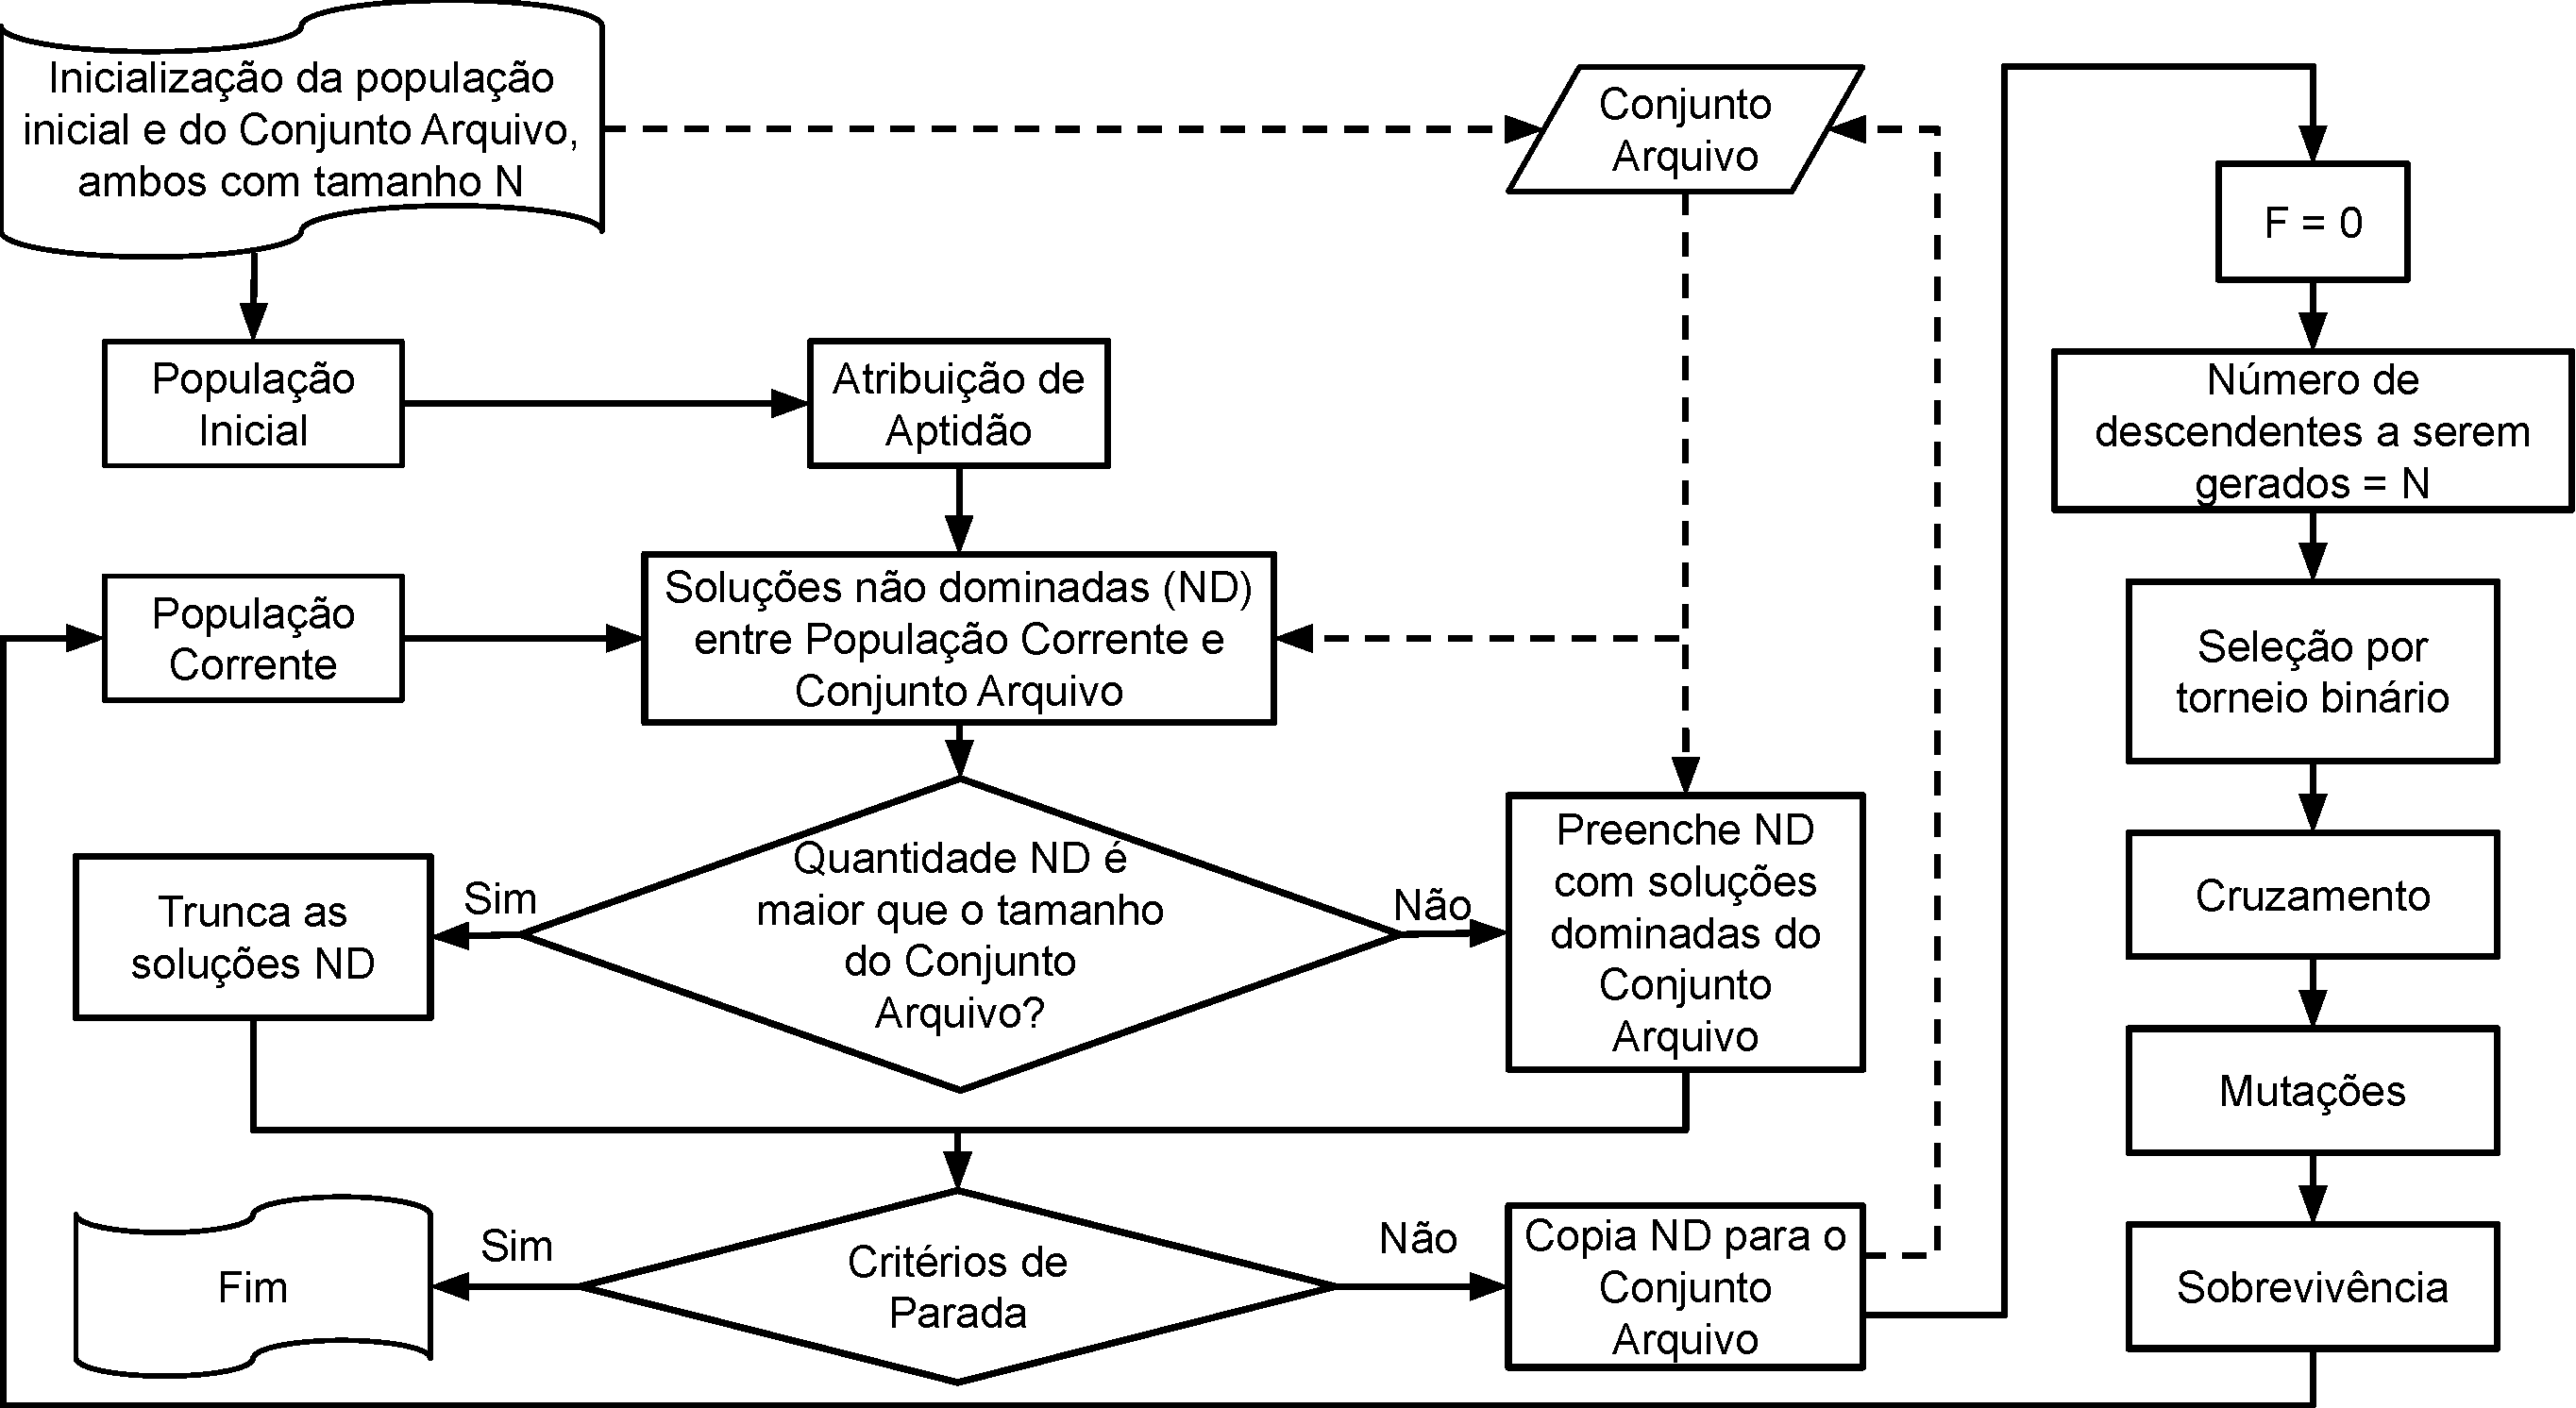
\includegraphics[width=0.8\textwidth]{fig/fluxo_spea2_pt.pdf}
\caption{Fluxograma do algoritmo SPEA2 mostrando as principais etapas de execução}
\label{fig:spea2_flow}
\end{figure}

Conforme apresentado na Figura~\ref{fig:spea2_flow}, o processo de evolução do SPEA2 pode ser resumido nos seguintes passos principais:

\begin{enumerate}
    \item \textbf{Inicialização:} A população inicial e o Conjunto Arquivo são inicializados, ambos com tamanho $N$. Esta etapa estabelece o ponto de partida para o processo evolutivo;
    
    \item \textbf{Atualização do Conjunto Arquivo:} Todos os indivíduos não dominados da população corrente $P_t$ e do Conjunto Arquivo $\bar{P}_t$ são identificados e copiados para formar um novo Conjunto Arquivo $\bar{P}_{t+1}$ para a próxima geração. Indivíduos dominados ou duplicatas (em termos de valores objetivo) são removidos durante esta operação;
    
    \item \textbf{Controle do tamanho do Conjunto Arquivo:} Se o número de soluções não dominadas for menor que o tamanho predefinido do Conjunto Arquivo, as posições restantes são preenchidas com as melhores soluções dominadas do Conjunto Arquivo anterior. Caso contrário, se o tamanho exceder o limite predefinido $\bar{N}$, os membros excedentes são removidos usando um método de truncamento que considera informações de densidade para preservar as características da fronteira não dominada;
    
    \item \textbf{Atribuição de aptidão:} Os valores de aptidão (baseados nas Equações~\ref{eq:strength_value}, \ref{eq:raw_fitness}, \ref{eq:density_estimation} e \ref{eq:final_fitness}) são calculados e atribuídos a todos os indivíduos tanto no Conjunto Arquivo quanto na população corrente;
    
    \item \textbf{Verificação dos critérios de finalização:} O algoritmo verifica se os critérios de parada foram atendidos (número máximo de gerações, convergência, etc.). Se atendidos, o processo é finalizado;
    
    \item \textbf{Seleção e reprodução:} Caso os critérios de finalização não sejam atendidos, operadores genéticos são aplicados para gerar a nova população $P_{t+1}$. A seleção por torneio binário é utilizada para escolher pais para reprodução, seguida pelos operadores de cruzamento e mutação para produzir $N$ descendentes que formarão a próxima geração.
\end{enumerate}

O fluxograma evidencia a natureza cíclica do algoritmo, onde o Conjunto Arquivo atua como um repositório elitista que preserva as melhores soluções encontradas ao longo do processo evolutivo, enquanto a população corrente é renovada a cada geração através dos operadores genéticos.

\subsection{Comparação com Outros MOEAs}

Ao comparar o SPEA2 com outros algoritmos evolutivos multi-objetivo notáveis, como o \textit{Non-dominated Sorting Genetic Algorithm II} (NSGA-II)~\cite{deb2002fast}, \textit{Multi-objective Particle Swarm Optimization} (MOPSO)~\cite{MOPSO} e \textit{Pareto Envelope-based Selection Algorithm II} (PESA-II)~\cite{PESA}, certas características distintivas se tornam evidentes.

Diferentemente do NSGA-II, o SPEA2 calcula explicitamente a força de cada indivíduo e utiliza um Conjunto Arquivo que está diretamente envolvido na avaliação da aptidão para todos os indivíduos. Enquanto o NSGA-II classifica suas soluções com base na ordenação por não dominância seguida pela distância de aglomeração (\textit{crowding distance}), a atribuição de aptidão do SPEA2 combina as relações de dominância de um indivíduo (via aptidão bruta $R(i)$) com uma medida de densidade baseada no $k$-ésimo vizinho mais próximo $D(i)$.

Comparado ao MOPSO, o SPEA2 adota uma abordagem mais tradicional da computação evolutiva, englobando operadores genéticos de cruzamento, mutação e seleção, em oposição à metodologia inspirada em enxames do MOPSO. Em contraste com a abordagem baseada em grade (\textit{grid-based}) do PESA-II para manter a diversidade, o SPEA2 preserva a diversidade populacional usando sua estimativa de densidade baseada no $k$-ésimo vizinho mais próximo.

Embora esses MOEAs possuam características únicas e vantagens específicas, a escolha entre eles frequentemente depende das particularidades do problema sendo abordado, incluindo o número de objetivos, dimensionalidade do espaço de busca e características da fronteira de Pareto.

O SPEA2 é reconhecido como um algoritmo robusto devido à sua capacidade de fornecer soluções de alta qualidade~\cite{zitzler2001spea2,citacaon1}. À medida que a otimização multi-objetivo se expande para diversos campos de aplicação, há uma demanda crescente por algoritmos de otimização mais eficazes~\cite{citacaon6}. No entanto, com o aumento da complexidade e escala dos problemas, torna-se necessário desenvolver abordagens eficientes que possam aproximar e distribuir soluções de forma mais rápida e eficaz próximo à fronteira de Pareto.

Diferentes técnicas podem ser incorporadas ou hibridizadas para contribuir com buscas locais ou globais, melhorando os resultados na resolução de problemas multi-objetivo. Uma abordagem promissora inclui a manutenção de um conjunto separado de soluções promissoras, como utilizado no próprio algoritmo SPEA2~\cite{zitzler2001spea2}. Algoritmos auxiliares também têm sido empregados para hibridizar algoritmos hospedeiros, intercalando buscas locais dentro do fluxo padrão de um algoritmo principal. Como exemplo de um algoritmo auxiliar usado nesses casos de hibridização, pode-se mencionar o método de Fertilização \textit{In Vitro} (IVF)~\cite{camilo-junior2011}.

\section{Hibridização de Algoritmos Evolutivos}
\label{sec:hibridizacao}

A hibridização de algoritmos evolutivos surgiu como uma abordagem fundamental para aprimorar o desempenho de técnicas de otimização em diversos domínios de problemas. Esta estratégia busca combinar características complementares de diferentes métodos para superar limitações individuais e melhorar tanto a qualidade das soluções obtidas quanto a eficiência computacional~\cite{talbi2002taxonomy}.

A integração de métodos distintos pode ocorrer de várias formas. Segundo Blum et al.~\cite{blum2011hybrid}, a hibridização pode ser classificada em três categorias principais: (i) \textbf{sequencial}, onde os algoritmos são aplicados um após o outro; (ii) \textbf{paralela}, com execução simultânea de diferentes algoritmos cooperando entre si; e (iii) \textbf{integrativa}, incorporando componentes específicos de um algoritmo dentro da estrutura de outro.

Talbi~\cite{citacaon2} propõe uma taxonomia mais abrangente para classificar hibridizações, considerando aspectos como nível de acoplamento (fraco ou forte), ordem de execução (sequencial ou paralela) e distribuição hierárquica dos algoritmos combinados. Esta taxonomia fornece um framework sistemático para o desenvolvimento e análise de algoritmos híbridos.

A combinação de algoritmos evolutivos com técnicas de busca local tem demonstrado resultados particularmente relevantes na literatura. Ishibuchi e Murata~\cite{ishibuchi1998multi} foram pioneiros nessa abordagem, propondo a integração sistemática de busca local em algoritmos genéticos multi-objetivo. Essa estratégia, posteriormente formalizada sob o termo ``algoritmos meméticos'', permite refinar soluções candidatas e acelerar a convergência para a fronteira de Pareto~\cite{knowles2000memetic}.

Estudos recentes demonstraram que abordagens híbridas podem superar significativamente algoritmos evolutivos convencionais em termos de qualidade da solução e velocidade de convergência~\cite{zhou2011multiobjective}. No entanto, o sucesso da hibridização depende criticamente da configuração adequada dos parâmetros de controle de ambos os algoritmos componentes e da estratégia de integração adotada~\cite{deb2012analyzing}. Além disso, é essencial considerar o equilíbrio entre exploração (\textit{exploration}) e explotação (\textit{exploitation}) para evitar convergência prematura ou perda de diversidade populacional.

\section{Método de Fertilização \textit{In Vitro}}
\label{sec:ivf}

O método de Fertilização \textit{In Vitro} (IVF)~\cite{camilo-junior2011} é um algoritmo auxiliar paralelo que pode ser integrado à fase de manipulação genética de um algoritmo hospedeiro, visando melhorar o desempenho do algoritmo original através da geração de indivíduos promissores. O IVF é inspirado no processo de reprodução assistida utilizado em laboratórios para produção de espécimes com características geneticamente superiores, funcionando como uma biotécnica reprodutiva aplicada para acelerar a produção de descendentes com propriedades desejáveis.

\subsection{Procedimento do Método IVF}

O funcionamento do método IVF segue um fluxo estruturado que permite sua integração harmoniosa com algoritmos evolutivos hospedeiros. A Figura~\ref{fig:ivf_flow} apresenta uma visão geral do processo, destacando as principais etapas de execução e suas interações.

\begin{figure}[htbp]
\centering
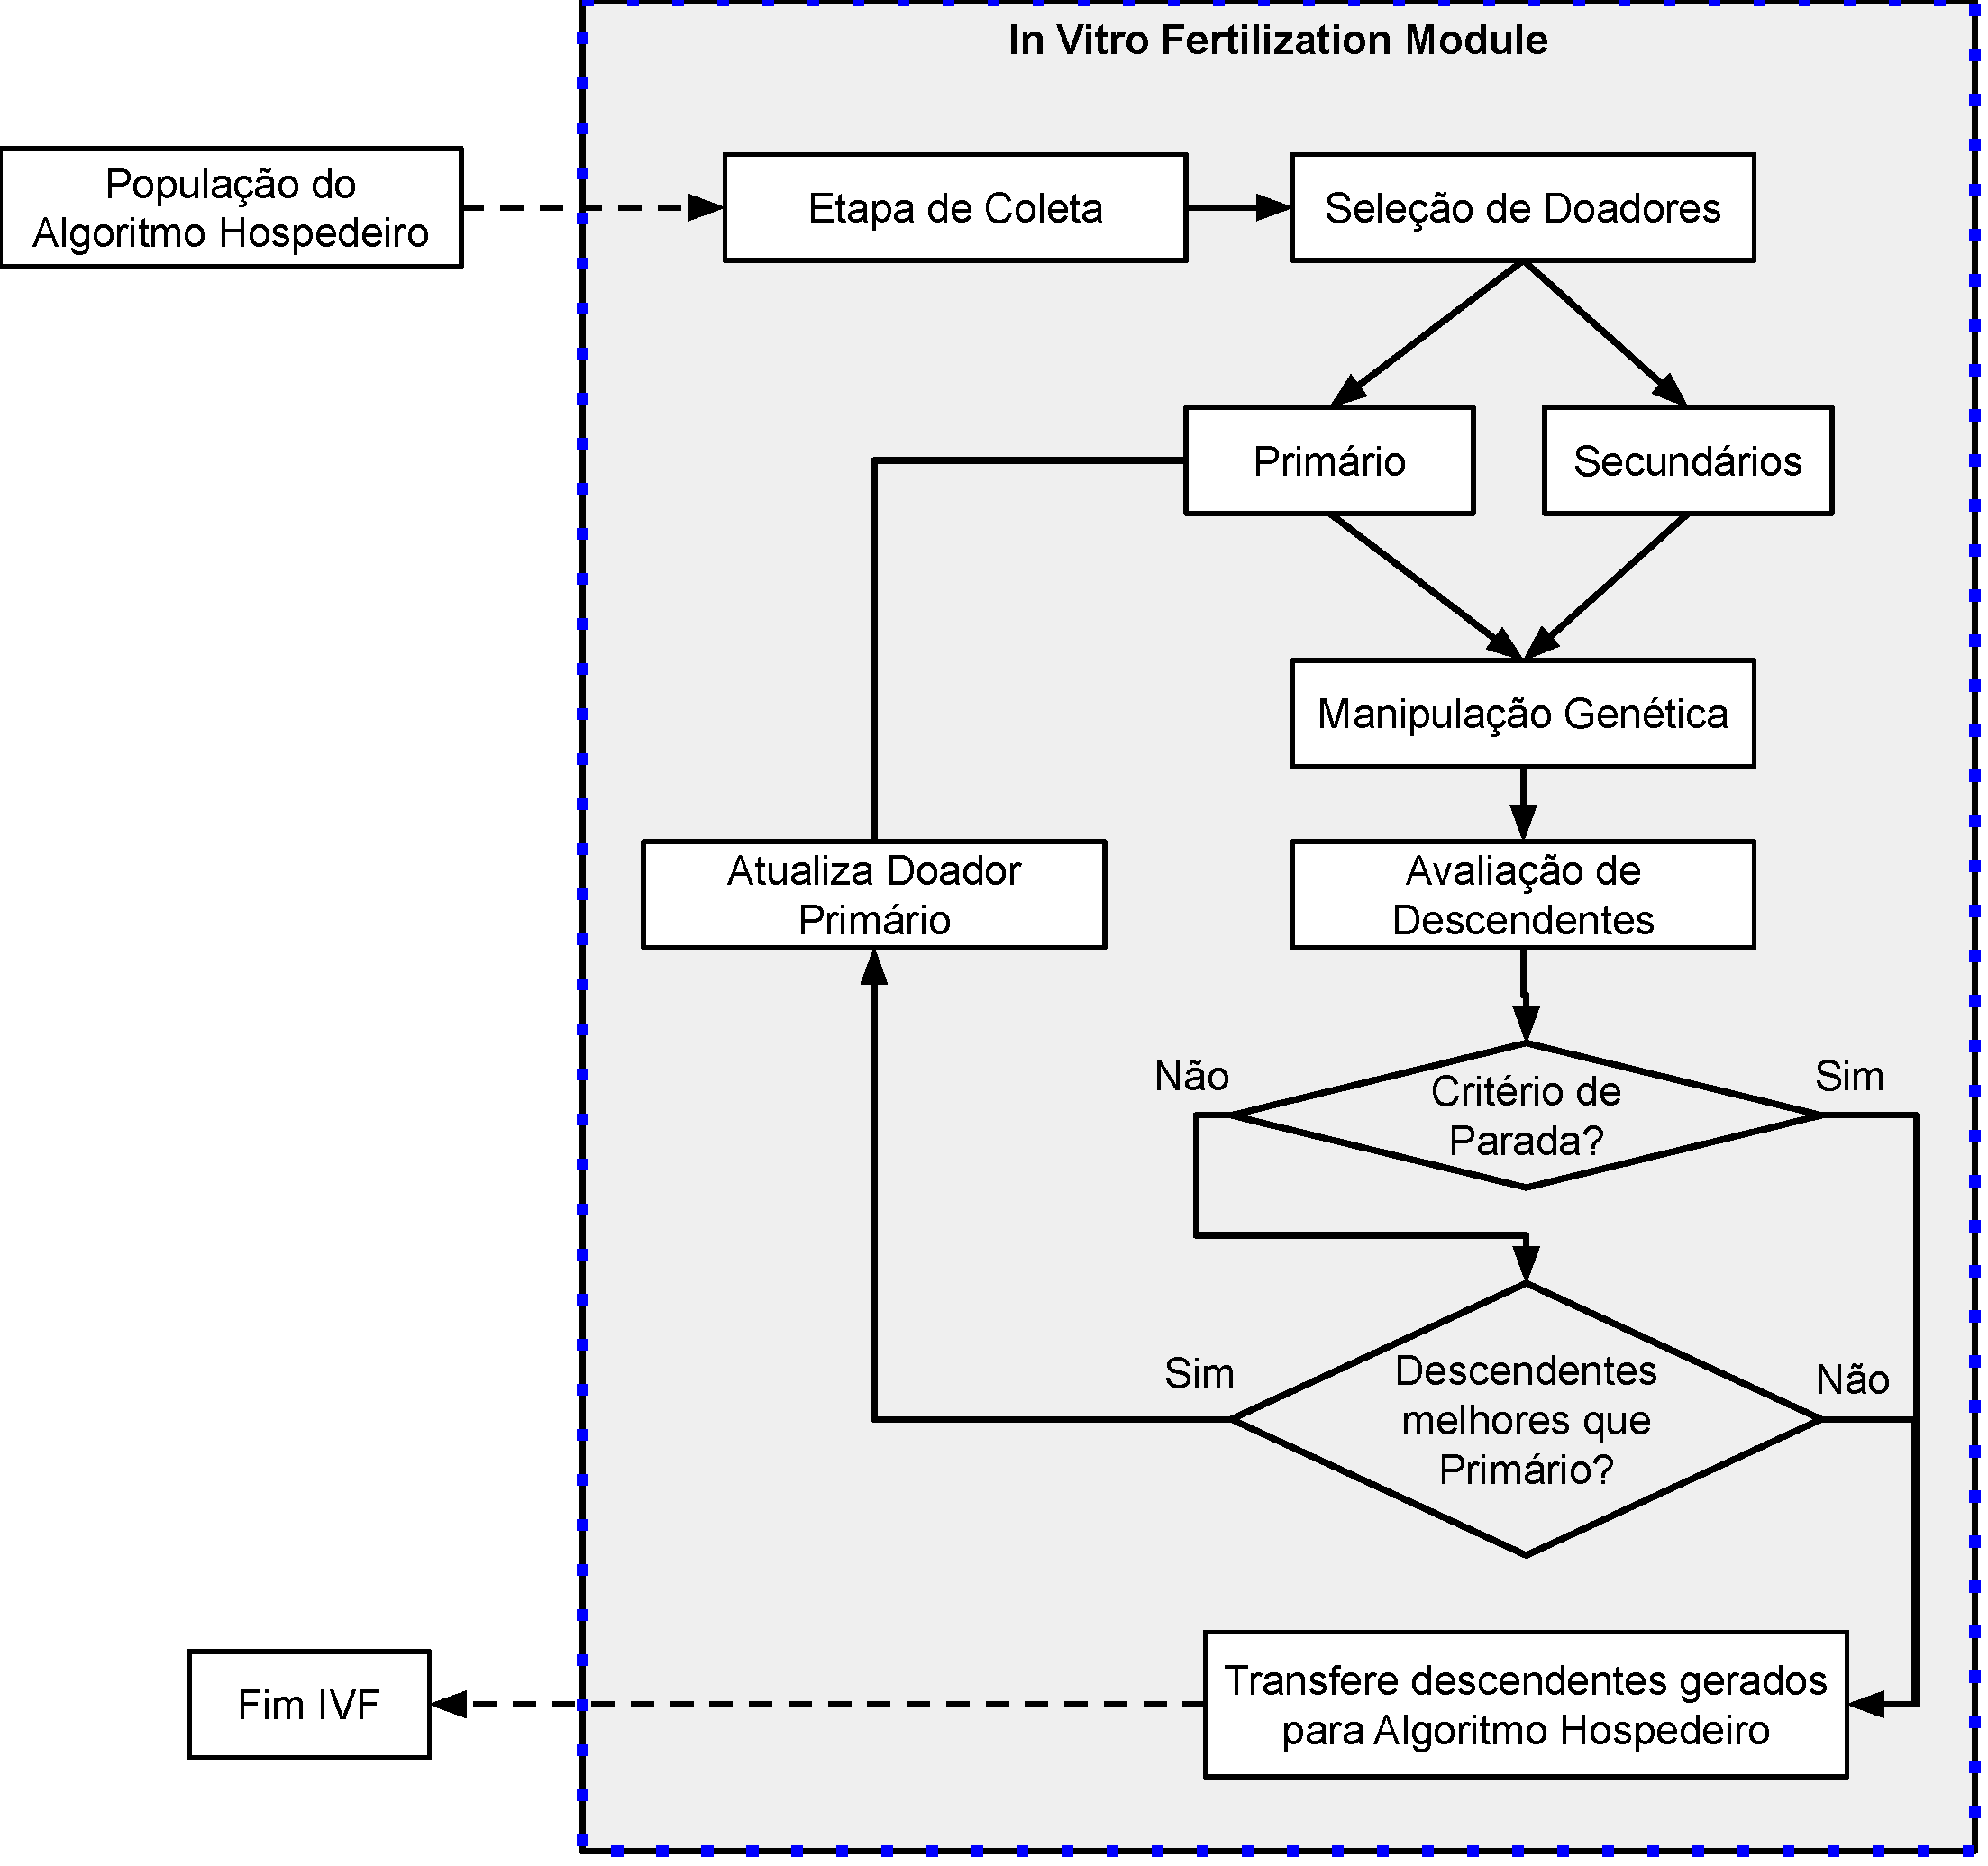
\includegraphics[width=0.7\textwidth]{fig/fluxo_ivf.pdf}
\caption{Fluxograma do método de Fertilização \textit{In Vitro} mostrando as etapas de coleta, manipulação genética e transferência}
\label{fig:ivf_flow}
\end{figure}

Conforme ilustrado na Figura~\ref{fig:ivf_flow}, o método IVF opera como um módulo independente que interage com o algoritmo hospedeiro através de três fases principais: coleta de material genético promissor, manipulação genética intensiva e transferência de descendentes superiores. O método IVF consiste nos seguintes passos principais:

\begin{enumerate}
    \item \textbf{Etapa de coleta:} Conforme mostrado na parte inicial do fluxograma, indivíduos promissores da população atual do algoritmo hospedeiro são coletados para manipulação genética. A seleção é baseada em critérios de qualidade definidos pelo problema, sendo que tipicamente $c$ indivíduos são coletados;
        
    \item \textbf{Separação de doadores:} O melhor indivíduo coletado é selecionado como o doador primário, enquanto os demais são designados como doadores secundários. Esta hierarquização permite direcionar as operações genéticas dentro do módulo de fertilização \textit{in vitro};
        
    \item \textbf{Manipulação genética:} Como destacado na figura, esta etapa central do processo aplica operações genéticas exploratórias, incluindo mutações direcionadas e cruzamentos elitistas, aos doadores coletados para criar descendentes com material genético promissor. O método IVF introduz variações controladas na composição genética, potencialmente gerando até $N$ indivíduos novos e superiores ($F \leq N$);
        
    \item \textbf{Avaliação da aptidão:} A aptidão dos descendentes é avaliada com base em seu desempenho nos objetivos do problema de otimização. Este passo fornece uma medida quantitativa da qualidade dos novos indivíduos gerados durante a manipulação genética;
        
    \item \textbf{Seleção de descendentes superiores:} Se um descendente superior emergir durante a fase de manipulação genética, superando a aptidão do doador primário atual, este indivíduo substitui o doador primário nas iterações subsequentes do método;
        
    \item \textbf{Critério de término:} Se nenhum descendente superar a aptidão do doador primário, ou outro critério de parada for atingido, o método IVF conclui suas iterações e prossegue para a fase de transferência;
        
    \item \textbf{Transferência:} Como ilustrado na etapa final da Figura~\ref{fig:ivf_flow}, um conjunto de $F$ descendentes superiores é transferido de volta para a população do algoritmo hospedeiro. Diferentes estratégias de transferência podem ser empregadas, incluindo a substituição de indivíduos menos aptos ou a expansão temporária da população.
\end{enumerate}

\subsection{Parâmetros de Controle}

O método IVF possui parâmetros específicos que controlam seu comportamento e integração com o algoritmo hospedeiro:

\begin{itemize}
    \item \textbf{Taxa de Execução ($r$):} Indica a probabilidade do método IVF ser acionado durante uma geração específica. Uma taxa mais alta resulta na execução do método IVF em um número maior de gerações, aumentando a intensidade da busca local;
    
    \item \textbf{Tamanho da Coleta ($c$):} Define o número de indivíduos coletados da população atual, incluindo o doador primário e os doadores secundários. Este parâmetro controla a diversidade genética disponível para manipulação.
\end{itemize}

\subsection{Operadores de Recombinação}

O método IVF emprega diferentes operadores de recombinação para explorar o espaço de busca de forma eficiente~\cite{camilo-junior2011}:

\begin{itemize}
    \item \textbf{Recombinação Assistida (AR):} Utiliza informações da população do algoritmo genético hospedeiro, aumentando a velocidade da operação sem realizar alterações genéticas significativas;
    
    \item \textbf{Recombinação Assistida Exploratória com Novos indivíduos (EAR-N):} Diversifica o espaço de busca substituindo metade dos doadores secundários por novos indivíduos gerados aleatoriamente;
    
    \item \textbf{Recombinação Assistida Exploratória Total (EAR-T):} Aplica mutação ao cromossomo completo de metade dos doadores secundários coletados, promovendo exploração ampla;
    
    \item \textbf{Recombinação Assistida Exploratória Parcial (EAR-P):} Realiza mutação em apenas parte do cromossomo dos doadores secundários, permitindo exploração localizada;
    
    \item \textbf{Recombinação Assistida Exploratória Parcial Adaptativa (EAR-PA):} Instiga mutação cromossômica parcial adaptativa em alguns indivíduos de metade dos doadores secundários, ajustando a intensidade da exploração conforme necessário.
\end{itemize}

Essas diferentes configurações de operadores permitem examinar sistematicamente a influência do método IVF no desempenho do algoritmo hospedeiro, possibilitando ajustes finos para diferentes tipos de problemas e características da fronteira de Pareto.
\chapter{Trabalhos Relacionados}
\label{sec:RW}
    O Algoritmo Genético com Fertilização In Vitro (IVF/GA)~\cite{camilo-junior2011} é uma extensão do algoritmo genético canônico que realiza busca local através de um processo denominado Fertilização In Vitro (IVF).

    Um estudo recente de Sampaio~\cite{sampaio2017ivf} apresentou uma abordagem diferente para o método IVF em otimização multiobjetivo. O estudo introduziu uma estratégia distinta para coletar indivíduos parentais iniciais, aprimorando a diversidade da população. No entanto, a estratégia de manipulação genética permaneceu inalterada, com apenas a melhor descendência substituindo o parental atual. Esta abordagem mantém os princípios fundamentais do método original e oferece oportunidades para a qualidade da solução.

    Publicações como IVF/NSGA-II~\cite{sampaio2017ivf} e IVF/GDE3~\cite{sampaio2019ivf} destacaram as contribuições positivas do acoplamento do método IVF com algoritmos evolutivos e de evolução diferencial populares como NSGA-II e GDE3. Estes trabalhos citados acima demonstraram o potencial do módulo para aprimorar as capacidades de convergência e diversificação do algoritmo hospedeiro. O acoplamento do método IVF com tais algoritmos fornece uma estrutura robusta para resolver problemas de otimização complexos e equilibrar o trade-off exploração-explotação.

    Além da hibridização direta com módulos de busca local como IVF, outros aprimoramentos significativos para MOEAs, incluindo SPEA2, têm se concentrado em adaptá-los a classes específicas de problemas desafiadores ou melhorar seus mecanismos centrais. Por exemplo, Problemas de Otimização Multiobjetivo com Restrições (CMOPs) apresentam consideráveis desafios quanto à satisfação de restrições e ao equilíbrio entre diversidade populacional e convergência. Para abordar isso, foi introduzido o framework de Otimização Multiforme (MFO), no qual o CMOP original é tratado juntamente com uma tarefa CMOP auxiliar em um cenário de otimização multitarefa~\cite{jiao2023multiform}. Quando implementado com SPEA2 (MFO-SPEA2), este framework não modifica intrinsecamente o algoritmo SPEA2 central, mas o integra em uma arquitetura de dupla tarefa adequada para CMOPs. A tarefa auxiliar, derivada do CMOP primário, opera com restrições inicialmente relaxadas que são dinamicamente e progressivamente restringidas. A transferência de conhecimento entre essas tarefas, uma forma implícita de hibridização de informações de busca, utiliza mecanismos de acasalamento e seleção personalizados para cada formulação de problema para guiar a busca evolutiva em direção a soluções Pareto-ótimas, aproveitando informações de domínios de soluções viáveis e inviáveis~\cite{jiao2023multiform}. Esta abordagem permitiu ao MFO-SPEA2 mostrar desempenho superior contra métodos representativos de tratamento de restrições e outros CMOEAs estado-da-arte em suítes de teste padrão e um problema real de síntese de arranjo de antenas~\cite{jiao2023multiform}.

    Dentro da otimização multi objetivos, algoritmos baseados em Pareto podem ter dificuldades devido à eficácia reduzida da relação de dominância de Pareto. Isso pode levar mecanismos de manutenção de diversidade a inadvertidamente guiar a busca para longe da verdadeira frente de Pareto~\cite{li2014shift}. Para abordar isso, a estratégia de Estimação de Densidade Baseada em Deslocamento (SDE) foi introduzida como uma melhoria ao componente de preservação de diversidade dos MOEAs~\cite{li2014shift}. SPEA2+SDE implementa esta estratégia modulando a estimação de densidade do k-ésimo vizinho mais próximo do SPEA2, efetivamente hibridizando o cálculo de densidade com informações de convergência~\cite{li2014shift}. SDE incorpora informações tanto distribucionais quanto relacionadas à convergência; durante a avaliação de densidade para um indivíduo focal, SDE computacionalmente ``desloca'' as posições de outros indivíduos baseado em suas características de convergência relativas ao indivíduo focal. Assim, soluções mal convergidas são percebidas como estando em regiões mais densas, diminuindo sua probabilidade de seleção~\cite{li2014shift}. Avaliações empíricas mostraram que SPEA2+SDE supera marcadamente o desempenho do SPEA2 canônico em problemas de otimização de muitos objetivos, especialmente conforme a dimensionalidade do espaço objetivo aumenta. Também demonstrou competitividade robusta contra outros algoritmos líderes projetados para cenários de muitos objetivos, destacando a eficácia desta modificação direcionada~\cite{li2014shift}. O estimador do k-ésimo vizinho mais próximo, integral ao SPEA2, é considerado particularmente propício à integração sinérgica com a metodologia SDE para desempenho aprimorado em muitos objetivos~\cite{li2014shift}.

    Avanços no método de Fertilização In Vitro e aumentações algorítmicas correlatas, como MFO e SDE, mostram promessa para alcançar resultados superiores em otimização multiobjetivo e de muitos objetivos. A confluência do projeto arquitetônico modular (como visto em hibridizações baseadas em IVF), estratégias de manipulação genética e adaptabilidade a domínios de problemas torna essas abordagens de hibridização opções atraentes dentro do conjunto de ferramentas de computação evolutiva. Concomitantemente, frameworks como MFO e técnicas exemplificadas por SDE fornecem mecanismos potentes para amplificar as capacidades operacionais de algoritmos bem estabelecidos, incluindo SPEA2, equipando-os assim para abordar efetivamente paisagens de otimização multiobjetivo novas e formidáveis.
\chapter{Proposta}
\label{sec:Proposal}

Aproveitando os princípios do método IVF apresentados na Seção~\ref{sec:ivf}, como manipulação genética e melhoramento seletivo, é possível explorar formas de melhorar a convergência e a diversidade das soluções geradas~\cite{camilo-junior2011}. O uso desses recursos pode resultar em soluções de maior qualidade que capturam melhor os compromissos entre diferentes objetivos em problemas de otimização multi-objetivo.

Os parâmetros do IVF, como a Taxa de Execução~``$r$'' e o Tamanho da Coleta~``$c$'', governam o equilíbrio entre a geração de novos indivíduos e a intensidade das manipulações genéticas internas. Ambos são projetados para serem controlados pelo operador com base nas necessidades ou características específicas do problema. Estudos e experimentações anteriores sugerem valores padrão para esses parâmetros. Por exemplo, uma Taxa de Execução~``$r$'' é frequentemente definida em torno de 10\% com base em trabalhos fundamentais do IVF~\cite{sampaio2017ivf, sampaio2019ivf}. A calibração de~``$r$'' é particularmente crucial, pois define a frequência de intervenção do IVF. Essa modulação cuidadosa da influência do módulo é essencial para garantir que ele contribua positivamente para o processo de otimização, apoiando, em vez de interromper, a evolução da população principal na busca por soluções ótimas.

Similarmente, o Tamanho da Coleta~``$c$'', que dita a quantidade de material genético coletado que entra no processo de melhoramento seletivo do módulo, também frequentemente assume um valor padrão em torno de 10\% do tamanho da população principal, com base em evidências empíricas de estudos anteriores~\cite{sampaio2017ivf, sampaio2019ivf}. Este padrão sugerido para~``$c$'' visa encontrar um equilíbrio eficaz entre o aprimoramento da qualidade da solução e o gerenciamento do consumo de avaliações de função. Isso ocorre porque a magnitude de~``$c$'' impacta diretamente a carga computacional; um tamanho de coleta maior leva a um número maior de avaliações realizadas pelo algoritmo IVF auxiliar. De fato, empregar um~``$c$'' excessivamente grande pode ser contraproducente devido ao consumo elevado de avaliações, uma preocupação observada em trabalhos derivados que exploram a integração do IVF com outros algoritmos como NSGA-II e GDE3~\cite{sampaio2017ivf, sampaio2019ivf}. Portanto, embora um~``$c$'' maior implique que mais material genético é processado e potencialmente soluções mais diversas são geradas durante a execução do módulo, é imperativo considerar cuidadosamente seu impacto substancial no orçamento geral de avaliações.

Ao selecionar e alternar os valores dessas variáveis, podemos explorar diferentes formas de realizar a manipulação genética e adaptá-las de acordo com os requisitos e características específicas da otimização do problema tratado. Essa flexibilidade permite uma exploração abrangente de várias técnicas de manipulação genética dentro do método IVF, aumentando sua eficácia e adaptabilidade na resolução de problemas de otimização multi-objetivo. Reconhecendo os benefícios da hibridização de algoritmos evolutivos e observando diferentes características e um compromisso entre intensificação e exploração na versão canônica do SPEA2, vale a pena investigar o acoplamento do método IVF com o algoritmo SPEA2, que já alcança resultados superiores em alguns problemas em comparação com outros algoritmos evolutivos multi-objetivo~\cite{zitzler2000comparison,zitzler2001spea2}.

Portanto, a proposta deste trabalho, denominada IVF/SPEA2, preserva a integridade do fluxo operacional padrão do SPEA2, conforme delineado na literatura~\cite{zitzler2001spea2}. No entanto, um mecanismo de acoplamento integrativo~\cite{blum2011hybrid} é integrado no ponto de geração de novas soluções, como pode ser visto na Figura~\ref{fig:ivf_spea2_flow}. Dentro desta estrutura, a execução do método IVF em qualquer geração é contingente ao total de Avaliações de Função (FEs) consumidas até o momento. Consequentemente, o processo pelo qual o algoritmo hospedeiro (SPEA2) gera novos indivíduos deve ser adaptado para operar dentro de um orçamento predefinido ($N$) de FEs atribuído por geração.

\begin{figure*}[htbp]
\centering
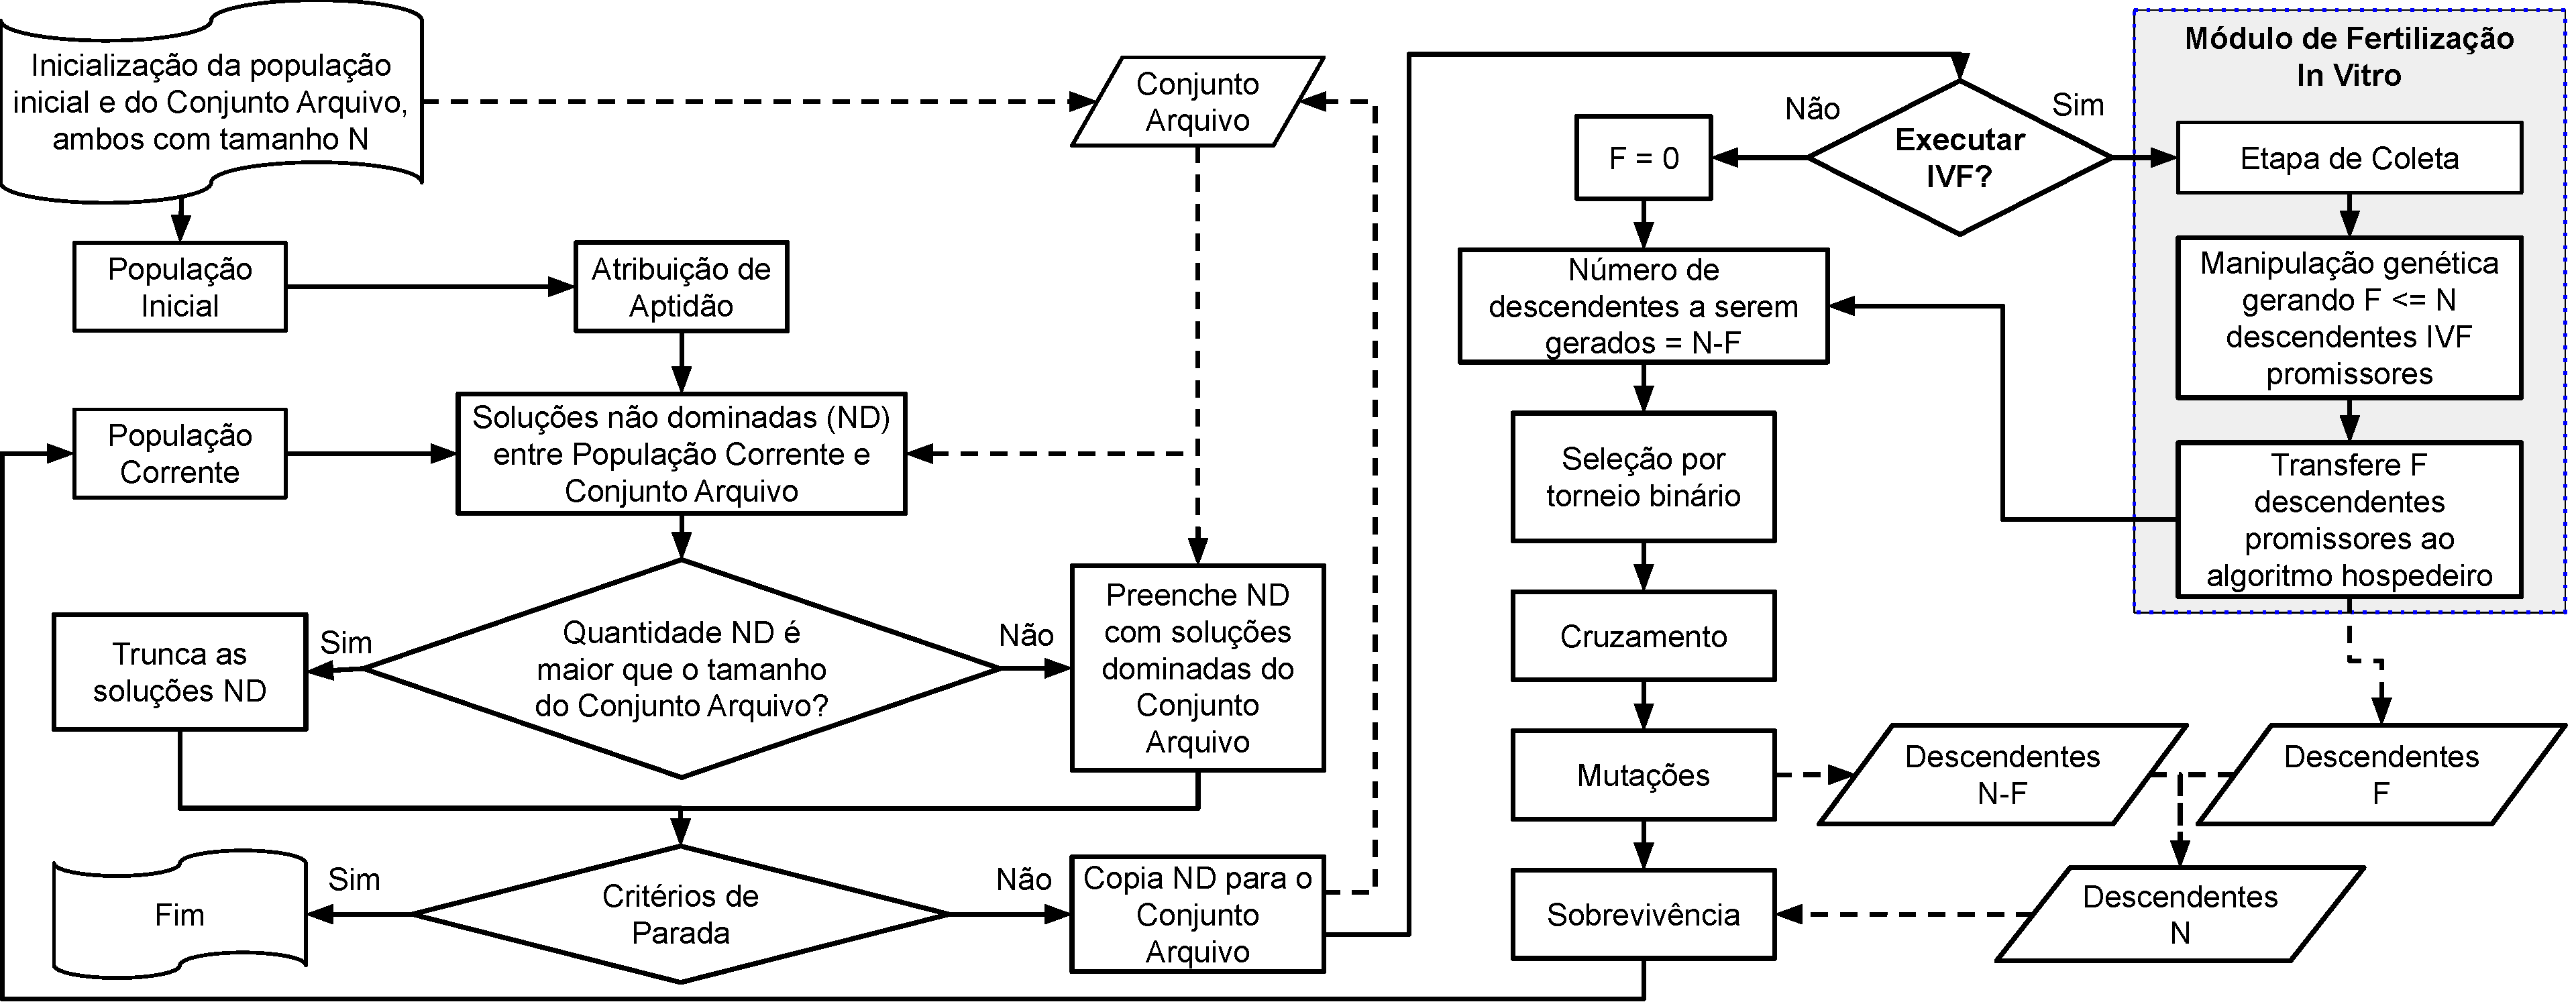
\includegraphics[width=\textwidth]{fig/fluxo_ivfspea2_pt.pdf}
\caption{O fluxo do algoritmo IVF/SPEA2. \textbf{Legenda:} Linhas contínuas representam o fluxo principal do algoritmo hospedeiro SPEA2; linhas tracejadas indicam fluxo condicional e integração do módulo IVF; a caixa com cor diferente destaca o Módulo de Fertilização \textit{In Vitro} como um componente adicional; setas bidirecionais mostram a troca de informações entre o algoritmo hospedeiro e o módulo IVF; nós de decisão (losangos) representam pontos de controle para as decisões do algoritmo.}
\label{fig:ivf_spea2_flow}
\end{figure*}

Na Figura~\ref{fig:ivf_spea2_flow}, pode-se observar o diagrama de fluxo de trabalho do algoritmo híbrido proposto (IVF/SPEA2). Seguindo os passos do algoritmo SPEA2, as operações básicas são fundamentadas da mesma forma, aderindo à filosofia evolutiva e elitista proposta por Zitzler et al.~\cite{zitzler2001spea2}. Visando a evolução e o equilíbrio entre diversificação e convergência, introduzimos o método IVF logo antes de gerar os descendentes tradicionais no fluxo hospedeiro, permitindo-nos gerar descendentes em número igual ao de indivíduos na população ao final de uma geração.

\section{Adaptações para a Integração com o SPEA2}

O principal diferencial do IVF/SPEA2 em comparação com acoplamentos anteriores (IVF/NSGA-II e IVF/GDE3) reside na adaptação da estratégia de comparação para determinar ciclos sucessivos no módulo IVF. No IVF/NSGA-II e IVF/GDE3, a comparação baseava-se na relação de dominância direta entre o indivíduo gerado e a(s) solução(ões) de elite atual(is), usando a dominância de Pareto para determinar se um novo ciclo deveria ser iniciado.

No entanto, considerando a estratégia específica do SPEA2, onde a melhor aptidão (menor valor numérico, já que $F(i)$ é minimizado conforme a Equação~\ref{eq:final_fitness}) nem sempre representa o indivíduo mais adequado na população uma vez que o $k$-ésimo vizinho mais próximo (onde $k = \lfloor\sqrt{N + \overline{N}}\rfloor$, conforme definido na Seção~\ref{sec:spea2}) é considerado ao calcular distâncias para outras soluções na estimativa de densidade (Equação~\ref{eq:density_estimation}), enquanto o NSGA-II examina o vizinho mais próximo usando a distância de aglomeração (\textit{crowding distance}) decidimos adaptar a abordagem para examinar se um novo indivíduo gerado no fluxo estava entre os $2 \times c$ indíviduos com menor valor para $F(i)$. Aqui, ``$c$'' representa o parâmetro de tamanho da coleta, e toda a população conhecida consiste em $N + \overline{N}$ indivíduos, onde $N$ é o tamanho da população principal e $\overline{N}$ é o tamanho do Conjunto Arquivo (ambos iguais a $N$ no SPEA2).

Essa modificação foi necessária devido à abordagem diferenciada do SPEA2 para o tratamento da densidade populacional em comparação com outros MOEAs. Enquanto o NSGA-II usa a distância de aglomeração considerando apenas o vizinho mais próximo para cálculos de densidade, o SPEA2 usa o $k$-ésimo vizinho mais próximo, onde a densidade é calculada como descrito na Equação~\ref{eq:density_estimation}. No SPEA2, a melhor aptidão (valor numericamente menor de $F(i)$) nem sempre indica o indivíduo mais adequado para seleção, pois considera a distribuição espacial das soluções no espaço objetivo, ao contrário do NSGA-II, onde uma melhor aptidão (baseada no \textit{ranking} de dominância e na distância de aglomeração) geralmente indica maior qualidade da solução.

A verificação da aptidão determina se a solução gerada está entre as $2 \times c$ melhores soluções (aquelas com os menores valores de $F(i)$) de acordo com a função de aptidão do SPEA2 (Equação~\ref{eq:final_fitness}), onde $R(i)$ é a aptidão bruta baseada na força de dominância (Equação~\ref{eq:raw_fitness}), e $D(i)$ é a estimativa de densidade (Equação~\ref{eq:density_estimation}). Se essa condição for atendida, um novo ciclo se inicia, usando a solução derivada com a melhor aptidão (menor valor de $F(i)$) como doadora primária para operações subsequentes. Essa adaptação permite que o IVF/SPEA2 aproveite totalmente a lógica de aptidão do SPEA2, mantenha a consistência com a filosofia de seleção baseada em densidade do algoritmo hospedeiro e preserve as características específicas de diversidade e convergência do SPEA2.

\section{Estágios do Módulo IVF}

O método IVF opera através de quatro estágios distintos, cada um com papéis específicos no processo de otimização híbrida, conforme ilustrado na Figura~\ref{fig:ivf_spea2_flow}:

\subsection{Gatilho de Ativação}

O gatilho de ativação determina quando o módulo IVF deve ser executado durante o processo evolutivo. Este mecanismo é baseado no parâmetro~``$r$'', que representa a porcentagem do total de avaliações que o IVF consumirá. O gatilho é ativado de acordo com o número de Avaliações de Função (FE) utilizadas até o momento atual, permitindo que o fluxo permaneça inalterado por algumas gerações, mantendo o comportamento do SPEA2 canônico. Isso fornece controle refinado sobre a frequência da interferência do IVF, evitando o descarrilamento da evolução da população e permitindo a calibração da influência do IVF no processo global de otimização.

\subsection{Estágio de Coleta}

O estágio de coleta reúne material genético de alta qualidade da população atual para manipulação. Este processo envolve a seleção de soluções promissoras com base na aptidão do SPEA2 e é controlado pelo parâmetro~``$c$''(tamanho da coleta). Um valor maior de ``$c$'' resulta em mais avaliações realizadas e uma maior quantidade de material genético disponível para manipulação genética. O critério de seleção utiliza a função de aptidão do SPEA2 $F(i) = R(i) + D(i)$ (Equação~\ref{eq:final_fitness}), considerando tanto a dominância ($R(i)$) quanto a densidade ($D(i)$), garantindo a representatividade e a qualidade das soluções coletadas para o processo de fertilização \textit{in vitro}.

\subsection{Manipulação Genética}

O estágio de manipulação genética realiza operações genéticas especializadas no material coletado para gerar novos indivíduos promissores. As estratégias disponíveis incluem os diferentes operadores de recombinação descritos na Seção~\ref{sec:ivf}: modificações sutis em soluções conhecidas para intensificação (AR), geração de soluções completamente novas para diversificação (EAR-N), e alternância entre estratégias de acordo com as características do problema (EAR-T, EAR-P, EAR-PA). Essa flexibilidade permite a exploração abrangente de diferentes técnicas de manipulação genética, adaptação a necessidades específicas do problema e configurações personalizáveis de compromisso entre intensificação e exploração. O controle de qualidade limita a geração a $F \leq N$ indivíduos por ciclo, com múltiplos ciclos possíveis até que todas as avaliações alocadas sejam consumidas.

\subsection{Estágio de Transferência}

O estágio de transferência integra soluções superiores geradas pelo IVF ao algoritmo hospedeiro. O critério de transferência requer que as soluções estejam entre os $2 \times c$ melhores indivíduos (aqueles com os menores valores de $F(i)$) da população completa ($N + \overline{N}$ indivíduos), avaliadas com base na função de aptidão do SPEA2, garantindo que apenas material genético de alta qualidade seja transferido. O processo de integração transfere $F$ soluções superiores para o algoritmo hospedeiro enquanto ajusta o número de descendentes tradicionais para $N-F$, mantendo o tamanho da população consistente ($N$ indivíduos). Se uma solução derivada classificar-se entre as melhores, um novo ciclo é iniciado usando a solução derivada com a melhor aptidão (menor valor de $F(i)$) como doadora primária, permitindo potencialmente a transcendência de barreiras anteriormente intransponíveis na busca pela fronteira de Pareto ótima.

O método IVF opera com o parâmetro~``$r$'' que representa a porcentagem do total de avaliações que ele consumirá, permitindo que o fluxo permaneça inalterado por algumas gerações, como no SPEA2 canônico. Quando o método IVF é ativado e conclui sua execução, existe o potencial para que soluções promissoras derivadas de outras soluções de qualidade sejam integradas ao algoritmo hospedeiro (etapa de transferência), permitindo a transcendência de barreiras anteriormente intransponíveis e avançando ainda mais em direção à fronteira ótima de Pareto.

Dentro deste processo, múltiplos ciclos podem ocorrer, consumindo potencialmente todas as avaliações alocadas para a geração. Um novo ciclo se inicia quando uma solução derivada de soluções promissoras se classifica entre as melhores soluções da população. A comparação é baseada na aptidão da população conforme a função $F(i) = R(i) + D(i)$ do SPEA2, e é aqui que entra uma das principais adaptações projetadas para se alinhar melhor com a lógica de consideração de aptidão do SPEA2.

Através das diversas estratégias de manipulação genética do IVF, o elitismo pode ser aumentado ou reduzido ao longo das gerações, fazendo pequenas modificações em soluções coletadas conhecidas ou gerando soluções inteiramente novas. Isso cria novas configurações de compromisso  entre diversificação e intensificação, seguindo os princípios de hibridização de algoritmos evolutivos apresentados na Seção~\ref{sec:hibridizacao}. A abordagem visa facilitar a adaptação das configurações de intensificação e diversificação para otimizar domínios de problemas específicos, aproveitando as características complementares do SPEA2 e do método IVF.
\chapter{Experimentos}
\label{sec:Experiments}

Os experimentos foram conduzidos utilizando a plataforma PlatEMO~\cite{platemo} no MATLAB para comparar o algoritmo memético com os algoritmos estabelecidos SPEA2, MFO-SPEA2, SPEA2+SDE, NSGA-II, NSGA-III e MOEA/D. A avaliação englobou múltiplas suítes de benchmarks (ZDT, DTLZ, WFG e MaF), selecionadas por suas características complementares e níveis variados de complexidade:
\begin{itemize}
    \item \textbf{Benchmark ZDT}~\cite{zitzler2000comparison} oferece problemas com diferentes geometrias de fronteira de Pareto (convexa, côncava, desconectada).
    \item \textbf{Benchmark DTLZ}~\cite{deb2005scalable} estende a avaliação para objetivos escaláveis e dimensionalidade crescente.
    \item \textbf{Benchmark WFG}~\cite{huband2006review} introduz transformações criando geometrias complexas com características do mundo real (não-separabilidade, multimodalidade, assimetria).
    \item \textbf{Benchmark MaF}~\cite{cheng2017benchmark} fornece problemas de otimização com muitos objetivos que desafiam abordagens tradicionais~\cite{li2015many}.
\end{itemize}
Para fazer uma comparação justa alinhada com os padrões de pesquisa estabelecidos, empregamos a métrica de Distância Geracional Invertida (IGD). Este indicador de desempenho amplamente adotado mede tanto a convergência quanto a diversidade, calculando a distância entre as soluções na fronteira de Pareto obtida e um conjunto de referência representando a verdadeira fronteira ótima de Pareto. Valores menores de IGD indicam melhor desempenho do algoritmo, refletindo soluções que são bem distribuídas e mais próximas da fronteira ótima~\cite{bosman2003balance}.

Para validação estatística dos nossos resultados experimentais, implementamos o teste de soma de postos de Wilcoxon, um teste estatístico de hipótese não-paramétrico que avalia se duas amostras independentes provêm de populações com a mesma distribuição. Este teste é particularmente apropriado para comparar algoritmos de otimização, pois não faz suposições sobre a normalidade das distribuições dos dados. A significância estatística foi estabelecida no limiar convencional de $p < 0,05$, indicando que as diferenças observadas entre os desempenhos dos algoritmos eram improváveis de terem ocorrido apenas por acaso.

Devido à natureza estocástica do método proposto, para cada configuração de teste, o IVF/SPEA2 proposto e os algoritmos comparados SPEA2, MFO-SPEA2, SPEA2+SDE, NSGA-II, NSGA-III e MOEA/D foram cada um executados 100 vezes, com os dados de desempenho coletados usando a métrica IGD. Os algoritmos de benchmark utilizaram suas configurações de parâmetros padrão conforme definidas no PlatEMO versão 24.2.0.2923080 \cite{platemo}. Para o módulo IVF dentro do IVF/SPEA2 proposto, foram adotadas configurações padrão baseadas em estudos anteriores e descobertas experimentais \cite{sampaio2017ivf, sampaio2019ivf}, especificamente um Tamanho de Coleção ``c'' de 10\% do tamanho da população e uma Taxa de Execução ``r'' de 10\%.
\chapter{Resultados}
\label{sec:results}

A análise dos nossos resultados inicia-se com um resumo de alto nível do desempenho do IVF/SPEA2 em comparação com seu algoritmo base, o SPEA2, e outros algoritmos estabelecidos. O algoritmo IVF/SPEA2 foi configurado com parâmetros c = 10\% e r = 10\%, consistentes com trabalhos relacionados anteriores~\cite{Sampaio2024}, para avaliar seu impacto geral.

Para estabelecer as características fundamentais de desempenho da abordagem proposta, apresentamos primeiro uma comparação direta entre IVF/SPEA2 e seu algoritmo base SPEA2. A Tabela~\ref{tab:resumo} presenta o número de vitórias alcançadas por cada algoritmo em diferentes dimensionalidades do problema, com a proporção de vitórias calculada em relação ao número total de instâncias de teste. O critério de vitória baseia-se em melhorias estatisticamente significativas de acordo com o teste de soma de postos de Wilcoxon ($p<0,05$) aplicado aos valores da métrica IGD.

% Resumo dos resultados diretos
\begin{table}[!htb]
    \centering
    \caption{Resumo dos Resultados: IVF/SPEA2 vs SPEA2}
    \label{tab:resumo}
    \resizebox{0.75\textwidth}{!}{%
    \begin{tabular}{|l|c|c|c|c|}
        \hline
        \textbf{Número de} & \multicolumn{2}{c|}{\textbf{Vitórias}} & \multicolumn{2}{c|}{\textbf{Proporção (\%)}} \\
        \cline{2-5}
        \textbf{Objetivos} & \textbf{IVF/SPEA2} & \textbf{SPEA2} & \textbf{IVF/SPEA2} & \textbf{SPEA2} \\
        \hline
        M = 2 & 16 & 0 & 57,1\% & 0,0\% \\
        M = 3 & 14 & 3 & 60,9\% & 13,0\% \\
        \hline
    \end{tabular}
    }
\end{table}

Os resultados demonstram uma clara vantagem para a abordagem híbrida proposta, com o IVF/SPEA2 alcançando desempenho superior na maioria das instâncias de teste em ambos os cenários, não perdendo nenhuma comparação estatisticamente significativa no caso bi-objetivo, enquanto mantém forte desempenho no cenário tri-objetivo com aproximadamente 61\% das vitórias. Esta análise inicial estabelece a eficácia da estratégia de integração do IVF e fornece a base para estudos comparativos mais abrangentes.

Para contextualizar este desempenho dentro da paisagem mais ampla dos algoritmos de otimização multi-objetivo, expandimos nossa análise para incluir métodos estabelecidos da literatura. A Tabela~\ref{tab:maismenosigual_combinada} apresenta uma matriz de comparação abrangente mostrando os resultados estatísticos de vários algoritmos contra o SPEA2 como linha de base de referência. Cada entrada representa o número de vitórias (+), derrotas (-) e empates (=) baseados no teste de soma de postos de Wilcoxon aplicado aos valores de IGD, fornecendo insight sobre a posição competitiva relativa de cada algoritmo em diferentes complexidades de problema.

% Resumo comparativo com outros algoritmos
\begin{table}[!htb]
  \centering
  \caption{Comparação de algoritmos vs. SPEA2 nos casos bi-objetivo (M=2) e tri-objetivo (M=3) usando IGD e o teste de soma de postos de Wilcoxon ($p<0,05$). Os símbolos denotam vitórias (+), derrotas (-) e empates (=) relativos ao SPEA2.}
  \label{tab:maismenosigual_combinada}
  \resizebox{0.65\textwidth}{!}{%
  \begin{tabular}{|l|c|c|}
    \hline
    \textbf{Algoritmo} & \textbf{M=2 (+/-/ =)} & \textbf{M=3 (+/-/ =)} \\ 
    \hline
    IVF/SPEA2  & 16/0/12 & 14/3/6    \\ 
    MFOSPEA2   &  3/1/24 &  2/3/18  \\ 
    SPEA2+SDE  &  0/28/0 &  4/18/1  \\ 
    NSGA-II   &  1/26/1 &  2/21/0  \\ 
    NSGA-III  & 18/8/2  &  4/18/1  \\ 
    MOEA/D    &  8/18/2 &  1/21/1  \\ 
    \hline
  \end{tabular}
  }
\end{table}

A análise comparativa revela que o IVF/SPEA2 exibe o desempenho positivo mais consistente contra a linha de base SPEA2 em ambas as dimensionalidades do problema. Embora o NSGA-III mostre forte desempenho no caso bi-objetivo com 18 vitórias, ele experimenta um declínio significativo no cenário tri-objetivo, alcançando apenas 4 vitórias contra 18 derrotas. Em contraste, o IVF/SPEA2 mantém desempenho robusto em ambos os casos, com 16 vitórias em M=2 e 14 vitórias em M=3, demonstrando características superiores de escalabilidade. Os algoritmos restantes, incluindo MFOSPEA2, SPEA2+SDE, NSGA-II e MOEA/D, mostram vantagem competitiva limitada, com a maioria exibindo predominância de derrotas ou empates contra a linha de base. Estes resultados estabelecem o IVF/SPEA2 como uma abordagem altamente competitiva que efetivamente aproveita o mecanismo IVF para aprimorar o desempenho de seu algoritmo base.

Para substanciar estas descobertas resumidas, apresentamos comparações experimentais detalhadas através de suítes de benchmark abrangentes. As Tabelas~\ref{tab:comparacao_2obj} e \ref{tab:comparacao_3obj} fornecem os resultados experimentais completos para problemas bi-objetivo e tri-objetivo, respectivamente, apresentando valores medianos da Distância Geracional Invertida (IGD) como métrica principal de desempenho. Os detalhes de configuração experimental incluem: a coluna ``Problem'' identificando a instância específica do benchmark, ``$N$'' indicando o tamanho da população, ``$M$" denotando o número de objetivos, ``$D$'' representando o número de variáveis de decisão, e ``$FE$'' especificando o número de avaliações de função. Para cada comparação de algoritmo, os símbolos ``+'', ``='', e ``$-$'' adjacentes aos valores métricos do IVF/SPEA2 indicam superioridade, equivalência ou inferioridade estatisticamente significativa relativa ao algoritmo canônico SPEA2, determinados através do teste de soma de postos de Wilcoxon ($p<0,05$).

% Tabela detalhada para 2 objetivos
\begin{table}[!htb]
    \centering
    \caption{Comparação de IGD (mediana) entre IVF/SPEA2 e outros algoritmos em problemas de benchmark com $M=2$ objetivos.}
    \label{tab:comparacao_2obj}
    \resizebox{\textwidth}{!}{%
    \begin{tabular}{|l|c|c|c|c|c|c|c|c|c|c|c|}
        \hline
        \textbf{Problema} & \textbf{N} & \textbf{M} & \textbf{D} & \textbf{FE} 
        & \textbf{IVF/SPEA2} & \textbf{MFOSPEA2} & \textbf{SPEA2SDE} 
        & \textbf{NSGAII} & \textbf{NSGAIII} & \textbf{MOEA/D} & \textbf{SPEA2} \\
        \hline
        ZDT1  & 100 & 2 & 30 & 100000 
          & 3,9091e-3\,+  & 3,9324e-3\,+  & 4,2415e-3\,$-$ 
          & 4,8135e-3\,$-$  & 3,8879e-3\,+  & 3,9895e-3\,$-$  & 3,9725e-3 \\
        ZDT2  & 100 & 2 & 30 & 100000 
          & 3,9041e-3\,=  & 3,9269e-3\,=  & 6,0190e-3\,$-$ 
          & 4,8843e-3\,$-$  & 3,8070e-3\,+  & 4,0017e-3\,$-$  & 3,9132e-3 \\
        ZDT3  & 100 & 2 & 30 & 100000 
          & 4,8535e-3\,+  & 4,8859e-3\,=  & 5,2992e-3\,$-$ 
          & 5,4302e-3\,$-$  & 6,1267e-3\,$-$  & 1,2082e-2\,$-$  & 4,9225e-3 \\
        ZDT4  & 100 & 2 & 10 & 100000 
          & 3,8438e-3\,+  & 3,8335e-3\,+  & 4,2477e-3\,$-$ 
          & 4,5402e-3\,$-$  & 3,8949e-3\,$-$  & 4,8355e-3\,$-$  & 3,8632e-3 \\
        ZDT6  & 100 & 2 & 10 & 100000 
          & 3,0782e-3\,+  & 3,0847e-3\,+  & 3,4256e-3\,$-$ 
          & 3,6734e-3\,$-$  & 3,0013e-3\,+  & 3,5386e-3\,$-$  & 3,0951e-3 \\
        \hline
        DTLZ1 & 100 & 2 & 6  & 100000 
          & 1,8274e-3\,+  & 1,8366e-3\,=  & 1,9998e-3\,$-$ 
          & 2,2062e-3\,$-$  & 1,7860e-3\,+  & 1,7866e-3\,+  & 1,8341e-3 \\
        DTLZ2 & 100 & 2 & 11 & 100000 
          & 4,1387e-3\,+  & 4,1742e-3\,=  & 9,6713e-3\,$-$ 
          & 5,1248e-3\,$-$  & 3,9660e-3\,+  & 3,9659e-3\,+  & 4,1810e-3 \\
        DTLZ3 & 100 & 2 & 11 & 100000 
          & 4,1941e-3\,+  & 4,2814e-3\,=  & 1,0069e-2\,$-$ 
          & 5,3101e-3\,$-$  & 4,2241e-3\,=  & 4,4009e-3\,=  & 4,2939e-3 \\
        DTLZ4 & 100 & 2 & 11 & 100000 
          & 4,1576e-3\,=  & 4,1664e-3\,=  & 9,8278e-3\,$-$ 
          & 5,2006e-3\,$-$  & 3,9662e-3\,+  & 3,9659e-3\,+  & 4,1648e-3 \\
        DTLZ5 & 100 & 2 & 11 & 100000 
          & 4,1432e-3\,+  & 4,1708e-3\,=  & 1,0040e-2\,$-$ 
          & 5,0335e-3\,$-$  & 3,9660e-3\,+  & 3,9659e-3\,+  & 4,1741e-3 \\
        DTLZ6 & 100 & 2 & 11 & 100000 
          & 4,0691e-3\,+  & 4,0862e-3\,=  & 9,5098e-3\,$-$ 
          & 5,6503e-3\,$-$  & 3,9660e-3\,+  & 3,9659e-3\,+  & 4,0931e-3 \\
        DTLZ7 & 100 & 2 & 21 & 100000 
          & 4,7817e-3\,=  & 4,7290e-3\,=  & 5,2461e-3\,$-$ 
          & 5,3784e-3\,$-$  & 5,1155e-3\,$-$  & 7,3954e-3\,$-$  & 4,7743e-3 \\
        \hline
        WFG1  & 100 & 2 & 11 & 100000 
          & 1,2123e-2\,+  & 1,0933e-1\,$-$  & 4,0805e-2\,$-$ 
          & 2,1513e-2\,+  & 9,6925e-2\,$-$  & 3,2948e-2\,$-$  & 2,9251e-2 \\
        WFG2  & 100 & 2 & 11 & 100000 
          & 1,1092e-2\,=  & 1,0983e-2\,= & 1,3551e-2\,$-$ 
          & 1,2888e-2\,$-$  & 1,3849e-2\,$-$  & 4,3051e-2\,$-$  & 1,1077e-2 \\
        WFG3  & 100 & 2 & 11 & 100000 
          & 1,1996e-2\,=  & 1,1975e-2\,=  & 1,3096e-2\,$-$ 
          & 1,4471e-2\,$-$  & 1,1343e-2\,+ & 1,3815e-2\,$-$  & 1,2036e-2 \\
        WFG4  & 100 & 2 & 11 & 100000 
          & 1,2761e-2\,+  & 1,2921e-2\,=  & 3,2335e-2\,$-$ 
          & 1,5283e-2\,$-$  & 1,2233e-2\,+  & 1,5896e-2\,$-$  & 1,2891e-2 \\
        WFG5  & 100 & 2 & 11 & 100000 
          & 6,3535e-2\,+  & 6,3653e-2\,=  & 7,5654e-2\,$-$ 
          & 6,5339e-2\,$-$  & 6,3370e-2\,+  & 6,9752e-2\,$-$  & 6,3653e-2 \\
        WFG6  & 100 & 2 & 11 & 100000 
          & 8,4645e-2\,=  & 8,5944e-2\,=  & 9,0430e-2\,$-$ 
          & 8,1863e-2\,=  & 8,2999e-2\,=  & 8,1766e-2\,=  & 7,6357e-2 \\
        WFG7  & 100 & 2 & 11 & 100000 
          & 1,3391e-2\,+  & 1,3672e-2\,=  & 3,2030e-2\,$-$ 
          & 1,6980e-2\,$-$  & 1,2234e-2\,+  & 1,5391e-2\,$-$  & 1,3713e-2 \\
        WFG8  & 100 & 2 & 11 & 100000 
          & 1,0741e-1\,=  & 1,0690e-1\,=  & 1,1317e-1\,$-$ 
          & 1,0893e-1\,$-$  & 1,0541e-1\,+ & 1,0875e-1\,$-$  & 1,0748e-1 \\
        WFG9  & 100 & 2 & 11 & 100000 
          & 1,6238e-2\,=  & 1,5510e-2\,=  & 3,2450e-2\,$-$ 
          & 1,8524e-2\,$-$  & 1,4531e-2\,+  & 3,0985e-2\,$-$  & 1,5919e-2 \\
        \hline 
        MaF1  & 100 & 2 & 11 & 100000 
          & 3,7724e-3\,+  & 3,8007e-3\,=  & 3,9789e-3\,$-$ 
          & 4,6277e-3\,$-$  & 3,5707e-3\,+  & 3,5706e-3\,+  & 3,8039e-3 \\
        MaF2  & 100 & 2 & 11 & 100000 
          & 2,1457e-3\,+  & 2,1783e-3\,=  & 2,3809e-3\,$-$ 
          & 2,7588e-3\,$-$  & 2,0068e-3\,+  & 2,0121e-3\,+  & 2,1890e-3 \\
        MaF3  & 100 & 2 & 11 & 100000 
          & 4,3975e-3\,=  & 4,3869e-3\,=  & 7,7584e-3\,$-$ 
          & 4,9079e-3\,$-$  & 6,4275e-3\,$-$  & 1,1239e-2\,$-$  & 4,2022e-3 \\
        MaF4  & 100 & 2 & 11 & 100000 
          & 1,2679e-2\,=  & 1,2608e-2\,=  & 4,0880e-2\,$-$ 
          & 1,5525e-2\,$-$  & 3,5083e-2\,$-$  & 1,8710e-1\,$-$  & 1,2665e-2 \\
        MaF5  & 100 & 2 & 11 & 100000 
          & 1,2946e-2\,=  & 1,2871e-2\,=  & 3,2827e-2\,$-$ 
          & 1,5951e-2\,$-$  & 1,2231e-2\,+  & 1,3102e-2\,$-$  & 1,2854e-2 \\
        MaF6  & 100 & 2 & 11 & 100000 
          & 4,0666e-3\,+  & 4,0761e-3\,=  & 1,0025e-2\,$-$ 
          & 4,9620e-3\,$-$  & 3,9661e-3\,+  & 3,9659e-3\,+  & 4,0892e-3 \\
        MaF7  & 100 & 2 & 21 & 100000 
          & 4,7520e-3\,=  & 4,7574e-3\,=  & 5,1753e-3\,$-$ 
          & 5,4252e-3\,$-$  & 5,1169e-3\,$-$  & 7,3810e-3\,$-$  & 4,7840e-3 \\
        \hline
    \end{tabular}%
    }
\end{table}

Os resultados detalhados bi-objetivo demonstram a eficácia consistente do IVF/SPEA2 através de paisagens de problemas diversas. Examinando os padrões de desempenho, o IVF/SPEA2 alcança melhorias estatisticamente significativas sobre o SPEA2 em 16 das 28 instâncias de teste, sem casos de deterioração significativa, confirmando a robustez da abordagem híbrida. Particularmente notável é o forte desempenho do algoritmo nos benchmarks clássicos ZDT e DTLZ, onde consistentemente iguala ou supera o desempenho da linha de base. Os resultados também revelam que o IVF/SPEA2 mantém desempenho competitivo contra algoritmos mais recentes a ele e populares na literatura, frequentemente alcançando resultados superiores ou equivalentes comparados ao NSGA-II, MOEA/D e outros métodos de referência, enquanto demonstra força particular no manuseio de paisagens multimodais complexas como aquelas encontradas nas suítes de teste WFG e MaF.

Para examinar as características de escalabilidade da abordagem proposta, estendemos a análise para cenários de otimização tri-objetivo. A Tabela~\ref{tab:comparacao_3obj} apresenta os resultados experimentais abrangentes para problemas tri-objetivo, mantendo o mesmo protocolo experimental e estrutura de análise estatística do caso bi-objetivo. O aumento da dimensionalidade dos objetivos impõe desafios adicionais para convergência e manutenção da diversidade, tornando esta análise crucial para entender as limitações e forças de desempenho do algoritmo em espaços objetivos de dimensão superior.

\begin{table}[!htb]
    \centering
    \caption{Comparação do IGD (mediana) entre IVF/SPEA2 e outros algoritmos em problemas de referência com $M=3$ objetivos.}
    \label{tab:comparacao_3obj}
    \resizebox{\textwidth}{!}{%
    \begin{tabular}{|l|c|c|c|c|c|c|c|c|c|c|c|}
        \hline
        \textbf{Problema} & \textbf{N} & \textbf{M} & \textbf{D} & \textbf{AF} 
        & \textbf{IVF/SPEA2} & \textbf{MFOSPEA2} & \textbf{SPEA2SDE} 
        & \textbf{NSGAII} & \textbf{NSGAIII} & \textbf{MOEA/D} & \textbf{SPEA2} \\
        \hline
        DTLZ1  & 100 & 3 & 7  & 100000 
          & 2.0112e-2\,=  & 2.0184e-2\,$-$  & 2.0574e-2\,$-$  
          & 2.7057e-2\,$-$  & 2.0570e-2\,$-$  & 2.0566e-2\,$-$  & 2.0140e-2 \\
        DTLZ2  & 100 & 3 & 12 & 100000 
          & 5.3965e-2\,+  & 5.4223e-2\,$-$  & 7.6732e-2\,=   
          & 6.9228e-2\,$-$  & 5.4464e-2\,$-$  & 5.4446e-2\,$-$  & 5.4229e-2 \\
        DTLZ3  & 100 & 3 & 12 & 100000 
          & 5.3168e-2\,+  & 5.3458e-2\,$-$  & 7.6058e-2\,=   
          & 6.9016e-2\,$-$  & 5.4699e-2\,$-$  & 5.4768e-2\,$-$  & 5.3419e-2 \\
        DTLZ4  & 100 & 3 & 12 & 100000 
          & 3.8805e-1\,=  & 1.5063e-1\,+  & 1.9838e-1\,=   
          & 6.7606e-2\,+  & 1.6540e-1\,+  & 1.9110e-1\,=  & 2.3156e-1 \\
        DTLZ5  & 100 & 3 & 12 & 100000 
          & 4.3156e-3\,+  & 1.2417e-2\,$-$  & 1.0011e-2\,= 
          & 5.2873e-3\,$-$  & 3.3906e-2\,$-$  & 4.4229e-3\,$-$  & 1.1774e-1 \\
        DTLZ6  & 100 & 3 & 12 & 100000 
          & 4.0831e-3\,=  & 4.0876e-3\,$-$  & 9.6308e-3\,=   
          & 5.8744e-3\,$-$  & 1.8730e-2\,$-$  & 3.3924e-2\,$-$  & 4.0834e-3 \\
        DTLZ7  & 100 & 3 & 22 & 100000 
          & 6.9223e-2\,+  & 6.0497e-2\,=  & 8.0552e-2\,=   
          & 8.2232e-2\,$-$  & 8.1043e-2\,$-$  & 2.0871e-1\,$-$  & 7.4694e-2 \\
          \hline
        WFG1  & 100 & 3 & 12 & 100000 
          & 1.5019e-1\,+  & 1.5289e-1\,$-$  & 1.7729e-1\,= 
          & 2.2384e-1\,$-$  & 1.4904e-1\,+  & 2.2908e-1\,$-$  & 1.5277e-1 \\
        WFG2  & 100 & 3 & 12 & 100000 
          & 1.7885e-1\,-  & 1.6847e-1\,$-$  & 2.0638e-1\,+   
          & 2.2266e-1\,$-$  & 1.6469e-1\,+  & 2.3105e-1\,$-$  & 1.7229e-1 \\
        WFG3  & 100 & 3 & 12 & 100000 
          & 1.0839e-2\,+  & 1.0472e-2\,+  & 1.6581e-2\,$-$   
          & 1.5475e-2\,+  & 9.3581e-2\,$-$  & 1.6760e-2\,$-$  & 1.5755e-2 \\
        WFG4  & 100 & 3 & 12 & 100000 
          & 2.1409e-1\,+  & 2.1581e-1\,$-$  & 3.2292e-1\,=   
          & 2.6985e-1\,$-$  & 2.0092e-1\,$-$  & 2.5334e-1\,$-$  & 2.1540e-1 \\
        WFG5  & 100 & 3 & 12 & 100000 
          & 2.2190e-1\,+  & 2.2265e-1\,$-$  & 3.3187e-1\,=   
          & 2.7858e-1\,$-$  & 2.2989e-1\,$-$  & 2.4787e-1\,$-$  & 2.2289e-1 \\
        WFG6  & 100 & 3 & 12 & 100000 
          & 2.4118e-1\,=  & 2.4237e-1\,$-$  & 3.4176e-1\,=   
          & 3.0460e-1\,$-$  & 2.3889e-1\,=  & 2.7152e-1\,$-$  & 2.3991e-1 \\
        WFG7  & 100 & 3 & 12 & 100000 
          & 2.1575e-1\,+  & 2.1802e-1\,$-$  & 3.3027e-1\,= 
          & 2.7874e-1\,$-$  & 2.2109e-1\,$-$  & 2.9815e-1\,$-$  & 2.1710e-1 \\
        WFG8  & 100 & 3 & 12 & 100000 
          & 2.9318e-1\,+  & 2.9803e-1\,$-$  & 3.5941e-1\,$-$   
          & 3.7429e-1\,$-$  & 2.7899e-1\,+  & 3.0416e-1\,$-$  & 2.9546e-1 \\
        WFG9  & 100 & 3 & 12 & 100000 
          & 2.1691e-1\,-  & 2.9198e-1\,$-$  & 1.3367e-1\,= 
          & 2.7314e-1\,$-$  & 2.2159e-1\,$-$  & 2.6280e-1\,$-$  & 2.1642e-3 \\
        \hline
        MaF1  & 100 & 3 & 12 & 100000 
          & 4.1484e-2\,+  & 4.1895e-2\,$-$  & 4.2174e-2\,=   
          & 5.7330e-2\,$-$  & 6.0677e-2\,$-$  & 7.0475e-2\,$-$  & 4.1793e-2 \\
        MaF2  & 100 & 3 & 12 & 100000 
          & 3.2614e-2\,=  & 3.0998e-2\,+  & 3.1149e-2\,+   
          & 4.5892e-2\,$-$  & 3.6002e-2\,$-$  & 3.8947e-2\,$-$  & 3.2241e-2 \\
        MaF3  & 100 & 3 & 12 & 100000 
          & 3.2863e-2\,+  & 3.3571e-2\,$-$  & 5.8761e-2\,=   
          & 1.0803e-1\,$-$  & 4.7182e-2\,$-$  & 5.2002e-2\,$-$  & 3.3375e-2 \\
        MaF4  & 100 & 3 & 12 & 100000 
          & 2.4014e-1\,+  & 3.6409e-1\,$-$  & 3.6408e-1\,= 
          & 8.6124e-1\,$-$  & 4.0161e-1\,$-$  & 4.4124e-1\,$-$  & 3.6438e-3 \\
        MaF5  & 100 & 3 & 12 & 100000 
          & 1.5179e+0\,-  & 4.8561e-1\,$-$  & 8.3612e-1\,= 
          & 7.5943e-1\,$-$  & 8.5360e-1\,$-$  & 6.4408e-1\,+  & 7.8080e-1 \\
        MaF6  & 100 & 3 & 12 & 100000 
          & 4.0636e-3\,+  & 4.0809e-3\,$-$  & 9.7715e-3\,=   
          & 5.2715e-3\,$-$  & 1.5222e-2\,$-$  & 3.3929e-2\,$-$  & 4.0872e-3 \\
        MaF7  & 100 & 3 & 22 & 100000 
          & 7.4311e-2\,=  & 6.5112e-2\,$-$  & 5.9557e-2\,= 
          & 7.7718e-2\,$-$  & 9.6487e-2\,$-$  & 1.6567e-1\,$-$  & 7.4387e-2 \\
        \hline 
    \end{tabular}%
    }
\end{table}

Os resultados tri-objetivo revelam a competitividade mantida do IVF/SPEA2 apesar do aumento da complexidade da paisagem de otimização. O algoritmo alcança 14 melhorias estatisticamente significativas contra o SPEA2 nas 23 instâncias de teste, com apenas 3 casos mostrando deterioração e 6 empates, demonstrando notável resistência ao escalonamento dimensional. A análise do desempenho específico por problema de referência indica que o IVF/SPEA2 se destaca particularmente nos problemas DTLZ2, DTLZ3, DTLZ5 e DTLZ7, onde supera consistentemente o algoritmo de referência. Na desafiadora suíte WFG, o algoritmo mantém forte desempenho em WFG1, WFG3, WFG4, WFG5, WFG7 e WFG8, demonstrando sua capacidade de lidar com propriedades geométricas complexas e formas irregulares de frentes de Pareto. Os resultados do conjunto de referência MaF confirmam ainda mais a robustez do algoritmo, com melhorias notáveis em MaF1, MaF3, MaF4 e MaF6. Estes resultados abrangentes através de características de problemas diversas estabelecem o IVF/SPEA2 como uma abordagem escalável e robusta para otimização multi-objetivo, mantendo eficácia à medida que a complexidade dos problemas aumenta.

Para complementar os dados tabulares, uma análise visual abrangente de desempenho é apresentada através de representações em diagramas de caixa através de diferentes famílias de problemas de referência. As figuras seguintes utilizam valores normalizados de Distância Geracional Invertida (IGD) como métrica primária de desempenho, onde valores menores indicam desempenho superior do algoritmo. Cada diagrama de caixa exibe as características de distribuição incluindo mediana, quartis e valores discrepantes através de múltiplas execuções independentes, fornecendo insights sobre tanto a tendência central quanto a variabilidade de desempenho dos algoritmos avaliados.

\begin{figure}[!htb]
    \centering
    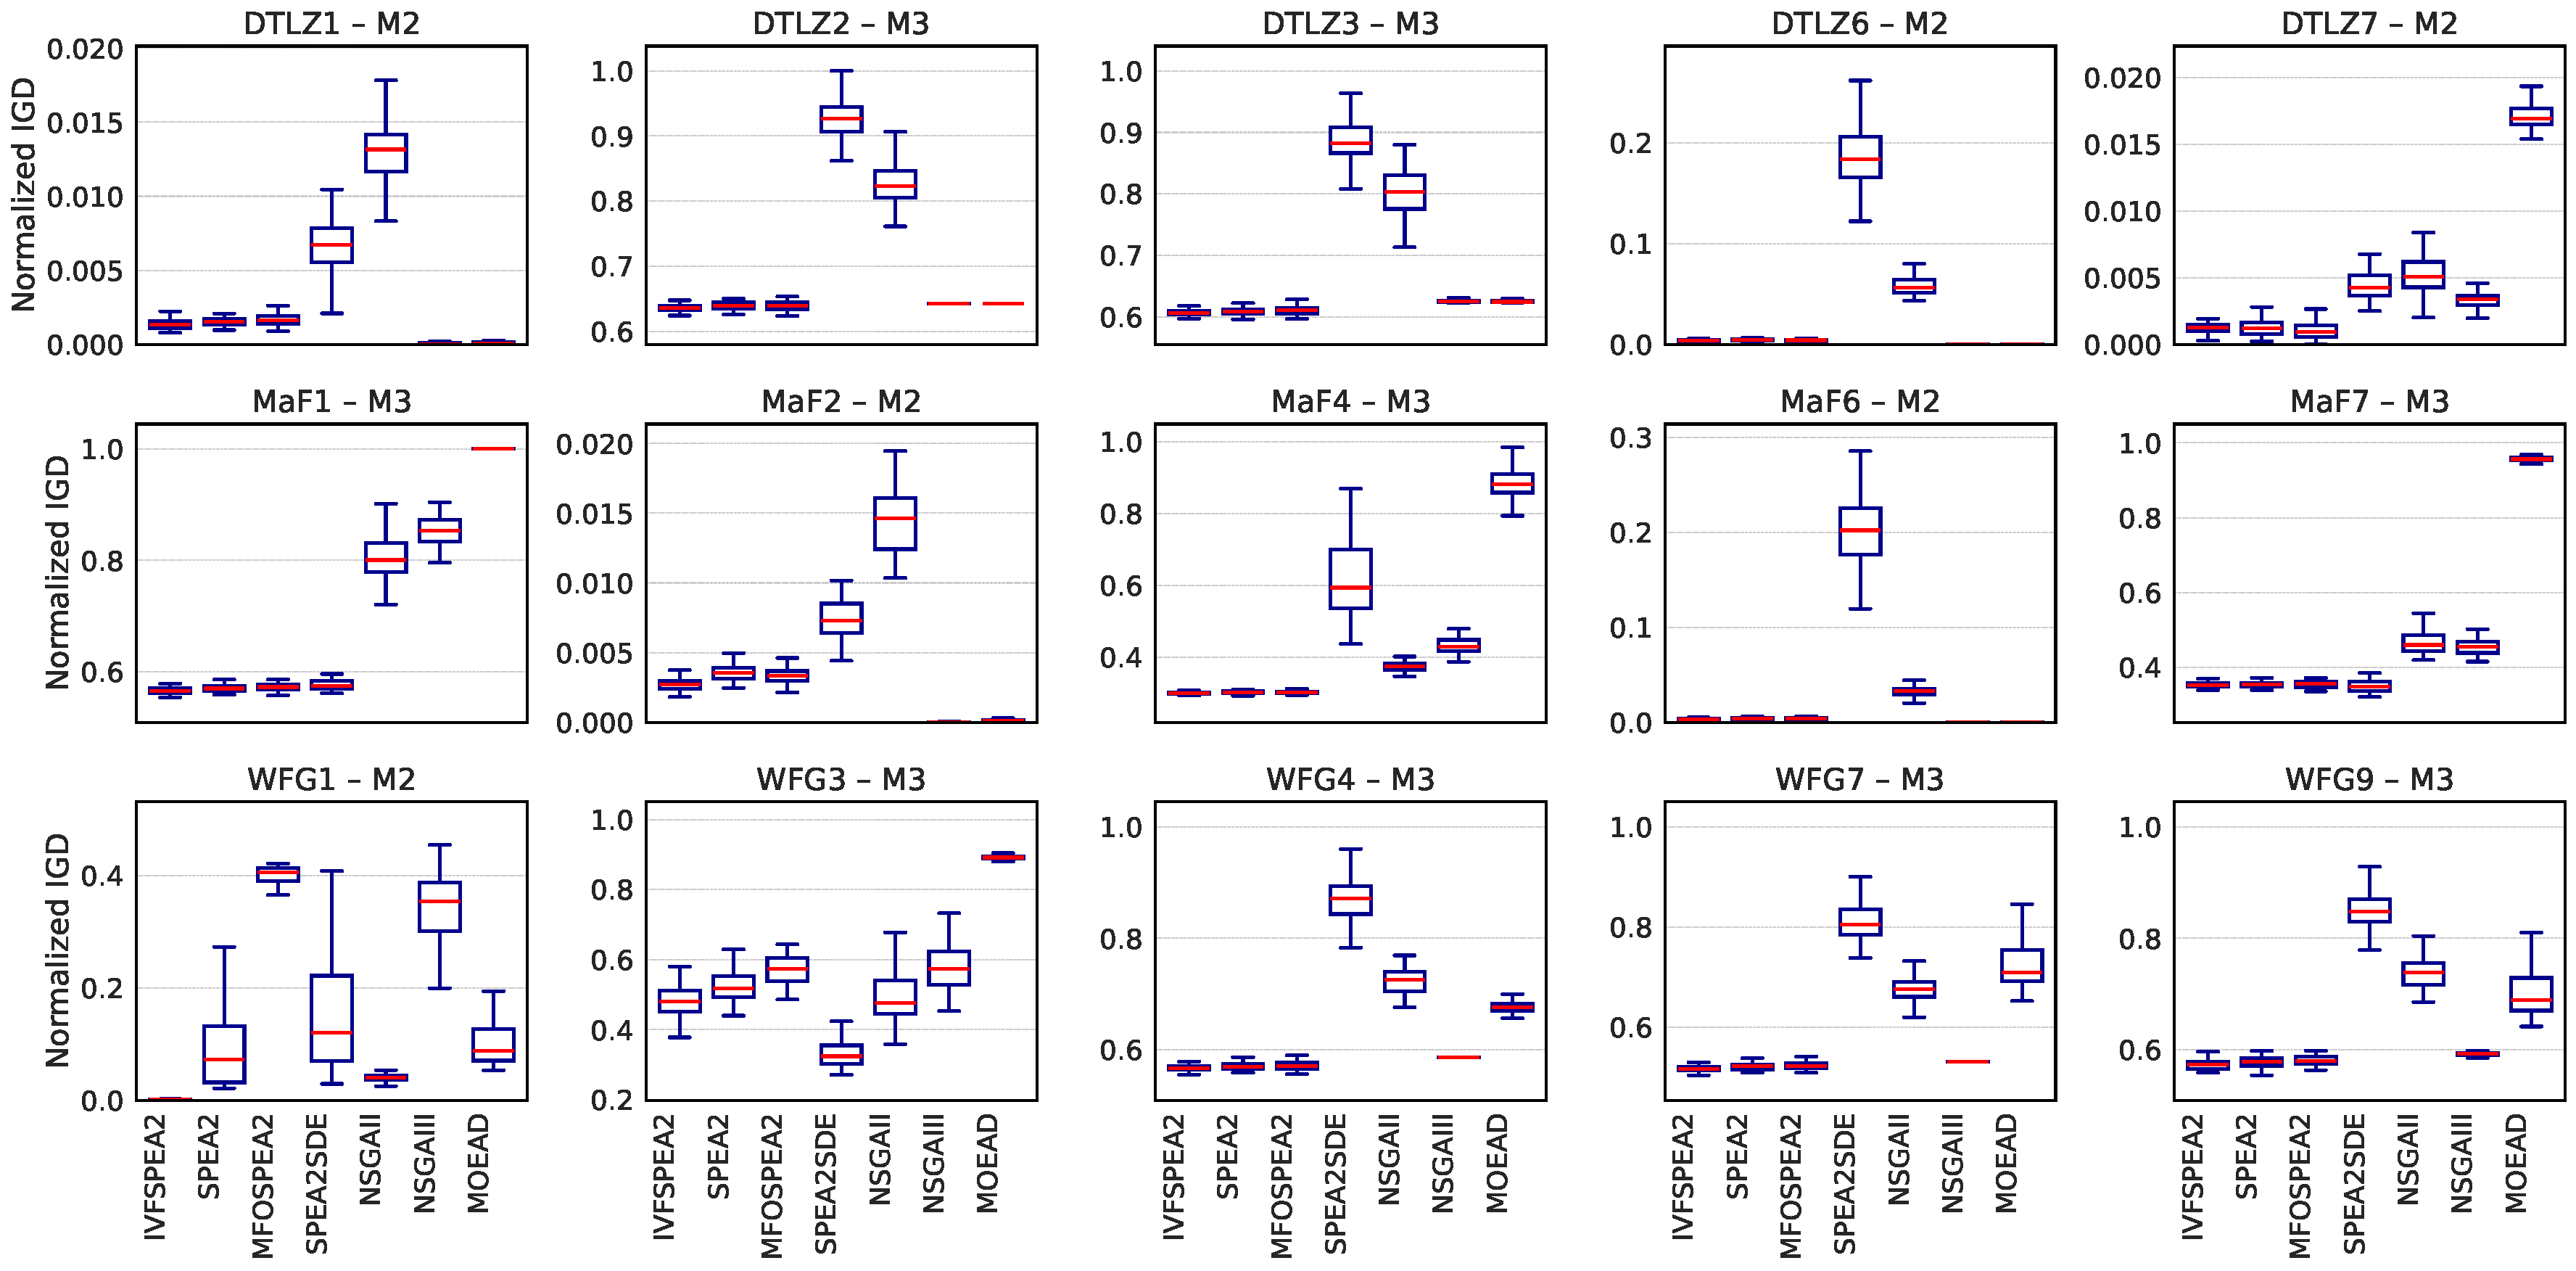
\includegraphics[width=\textwidth]{fig/boxplots_3x5_monocromatico_nome.pdf}
    \caption{Diagramas de caixa dos valores de IGD normalizado para problemas selecionados DTLZ, MaF e WFG, comparando IVF/SPEA2, SPEA2 e outros algoritmos de referência (MFOSPEA2, SPEA2SDE, NSGAII, NSGAIII, MOEAD).}
    \label{fig:boxplots_comparison}
\end{figure}

A análise dos diagramas de caixa na Figura~\ref{fig:boxplots_comparison} revela que o IVF/SPEA2 alcança consistentemente valores medianos de IGD menores na maioria dos problemas de referência, demonstrando qualidade de convergência superior. Particularmente notável é o desempenho do algoritmo em problemas desafiadores como DTLZ3 (M=3), MaF4 (M=3) e problemas WFG, onde o desempenho mediano e variância reduzida indicam tanto melhor qualidade de solução quanto estabilidade algorítmica aprimorada. Os problemas onde o IVF/SPEA2 demonstrou desempenho superior frequentemente compartilham características desafiadoras que testam a capacidade de um algoritmo de equilibrar convergência e diversidade:
\begin{itemize}
    \item \textbf{WFG1, WFG3-5, WFG7-9}: Características incluindo não-separabilidade, decepção, multimodalidade e geometrias complexas de frentes de Pareto~\cite{Huband2006}.
    \item \textbf{MaF1, MaF3, MaF6}: Paisagens complexas e interações objetivas desafiadoras~\cite{Cheng2017}.
    \item \textbf{DTLZ1, DTLZ2, DTLZ5, DTLZ6}: Várias geometrias de frentes de Pareto testando capacidades de convergência.
\end{itemize}

Para um exame mais detalhado do desempenho algorítmico dentro de famílias específicas de problemas de referência, a suíte de teste WFG é analisada separadamente devido à sua reputação por apresentar desafios de otimização diversos. A Figura~\ref{fig:wfg_igd_boxplot} apresenta distribuições de IGD normalizado para todos os nove problemas WFG, segregados por dimensionalidade do espaço objetivo. A comparação foca em três algoritmos chave: IVF/SPEA2, o SPEA2 de referência e MFOSPEA2 como um otimizador multi-objetivo representativo do estado da arte. Esta análise focada permite uma avaliação clara da consistência de desempenho através de problemas com características variadas como viés, não-separabilidade e paisagens enganosas.

\begin{figure}[!htb]
    \centering
    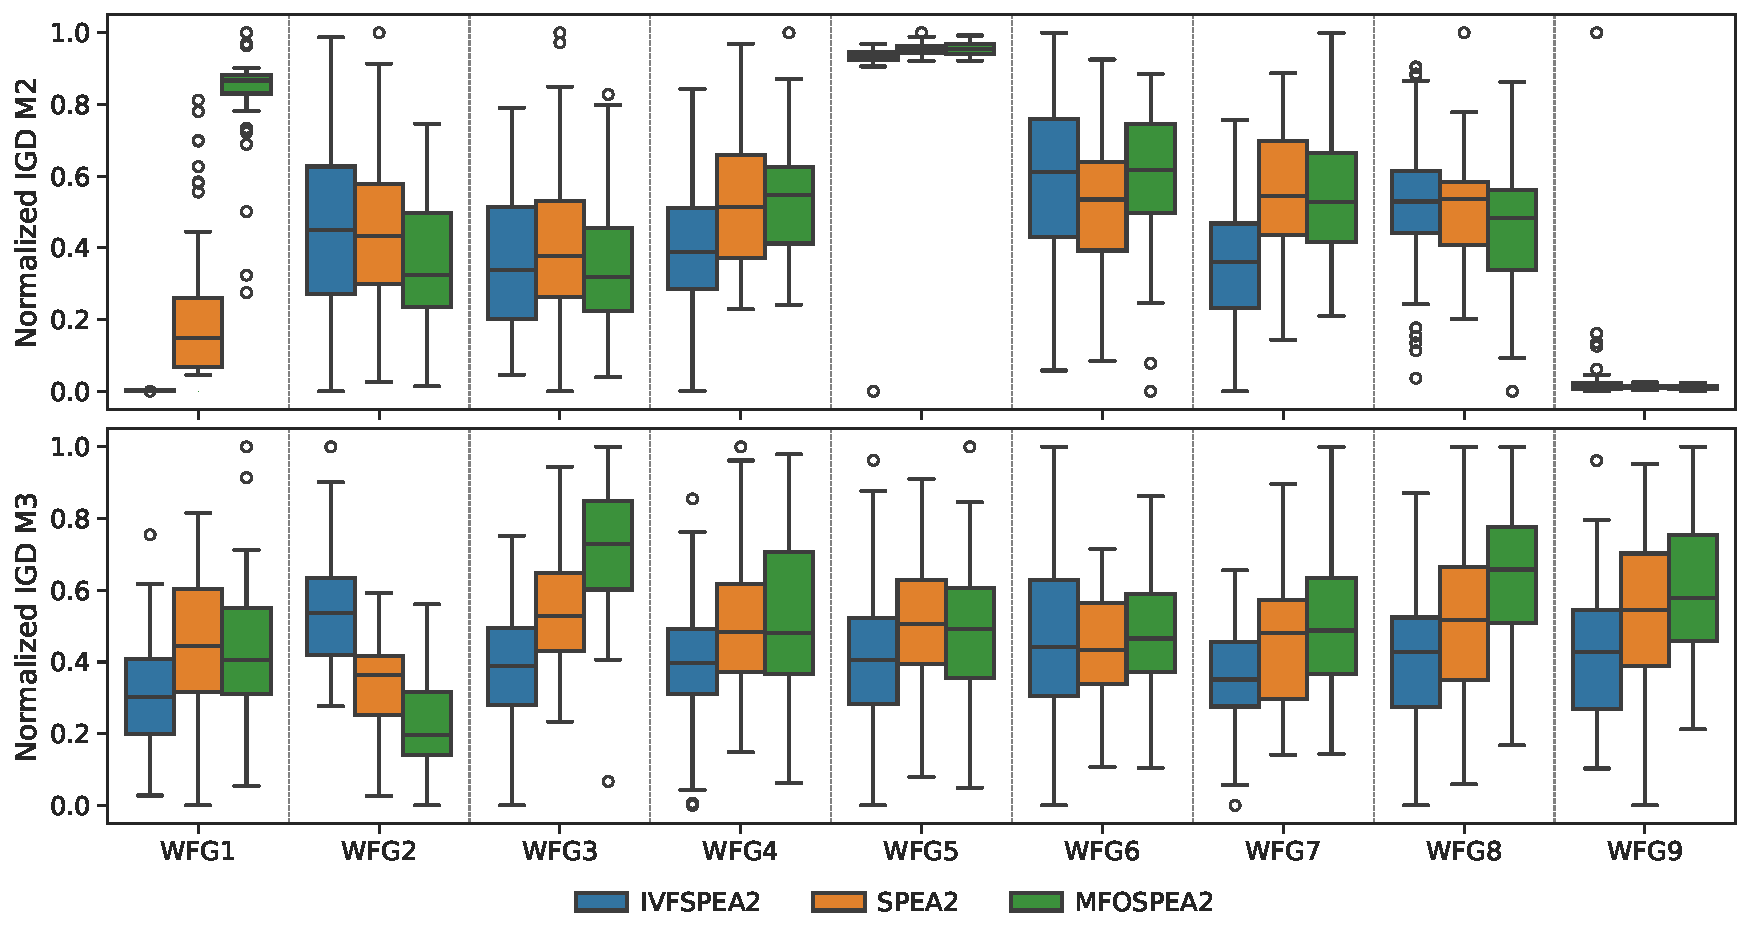
\includegraphics[
    %width=0.95\textwidth,
    height=0.25\textheight]{fig/wfg_igd_boxplot.pdf}
    \caption{Diagramas de caixa do IGD normalizado para problemas WFG (WFG1-WFG9) com M=2 e M=3 objetivos, comparando IVF/SPEA2, SPEA2 e MFOSPEA2. A linha superior exibe resultados para M=2 objetivos, e a linha inferior para M=3 objetivos.}
    \label{fig:wfg_igd_boxplot}
\end{figure}

A análise específica do WFG demonstra o desempenho robusto do IVF/SPEA2 através de toda a suíte, com vantagens particularmente pronunciadas em cenários tri-objetivo (M=3). O algoritmo exibe consistentemente valores medianos de IGD menores e intervalos interquartis reduzidos comparados tanto ao SPEA2 quanto ao MFOSPEA2. Este desempenho superior é especialmente evidente em WFG1, WFG3, WFG4 e WFG7, onde as características desafiadoras dos problemas como viés polinomial e variáveis de decisão não-separáveis tipicamente dificultam otimizadores multi-objetivo convencionais.

Para fornecer uma visão abrangente através de múltiplas famílias de problemas de referência, a Figura~\ref{fig:all_benchmarks_igd_boxplot} apresenta as distribuições de desempenho para as suítes de teste ZDT, DTLZ e MaF. Cada subgráfico representa uma família distinta de problemas de referência, com separação clara entre instâncias de problemas bi-objetivo (M=2) e tri-objetivo (M=3). Os três algoritmos comparados representam paradigmas algorítmicos diferentes: IVF/SPEA2 (abordagem proposta), SPEA2 (método clássico baseado em Pareto) e MFOSPEA2 (variante aprimorada do SPEA2 com gestão melhorada de diversidade). Esta estrutura comparativa permite a avaliação da robustez algorítmica através de diferentes paisagens de problemas e dimensionalidades do espaço objetivo.

\begin{figure}[!htb]
    \centering
    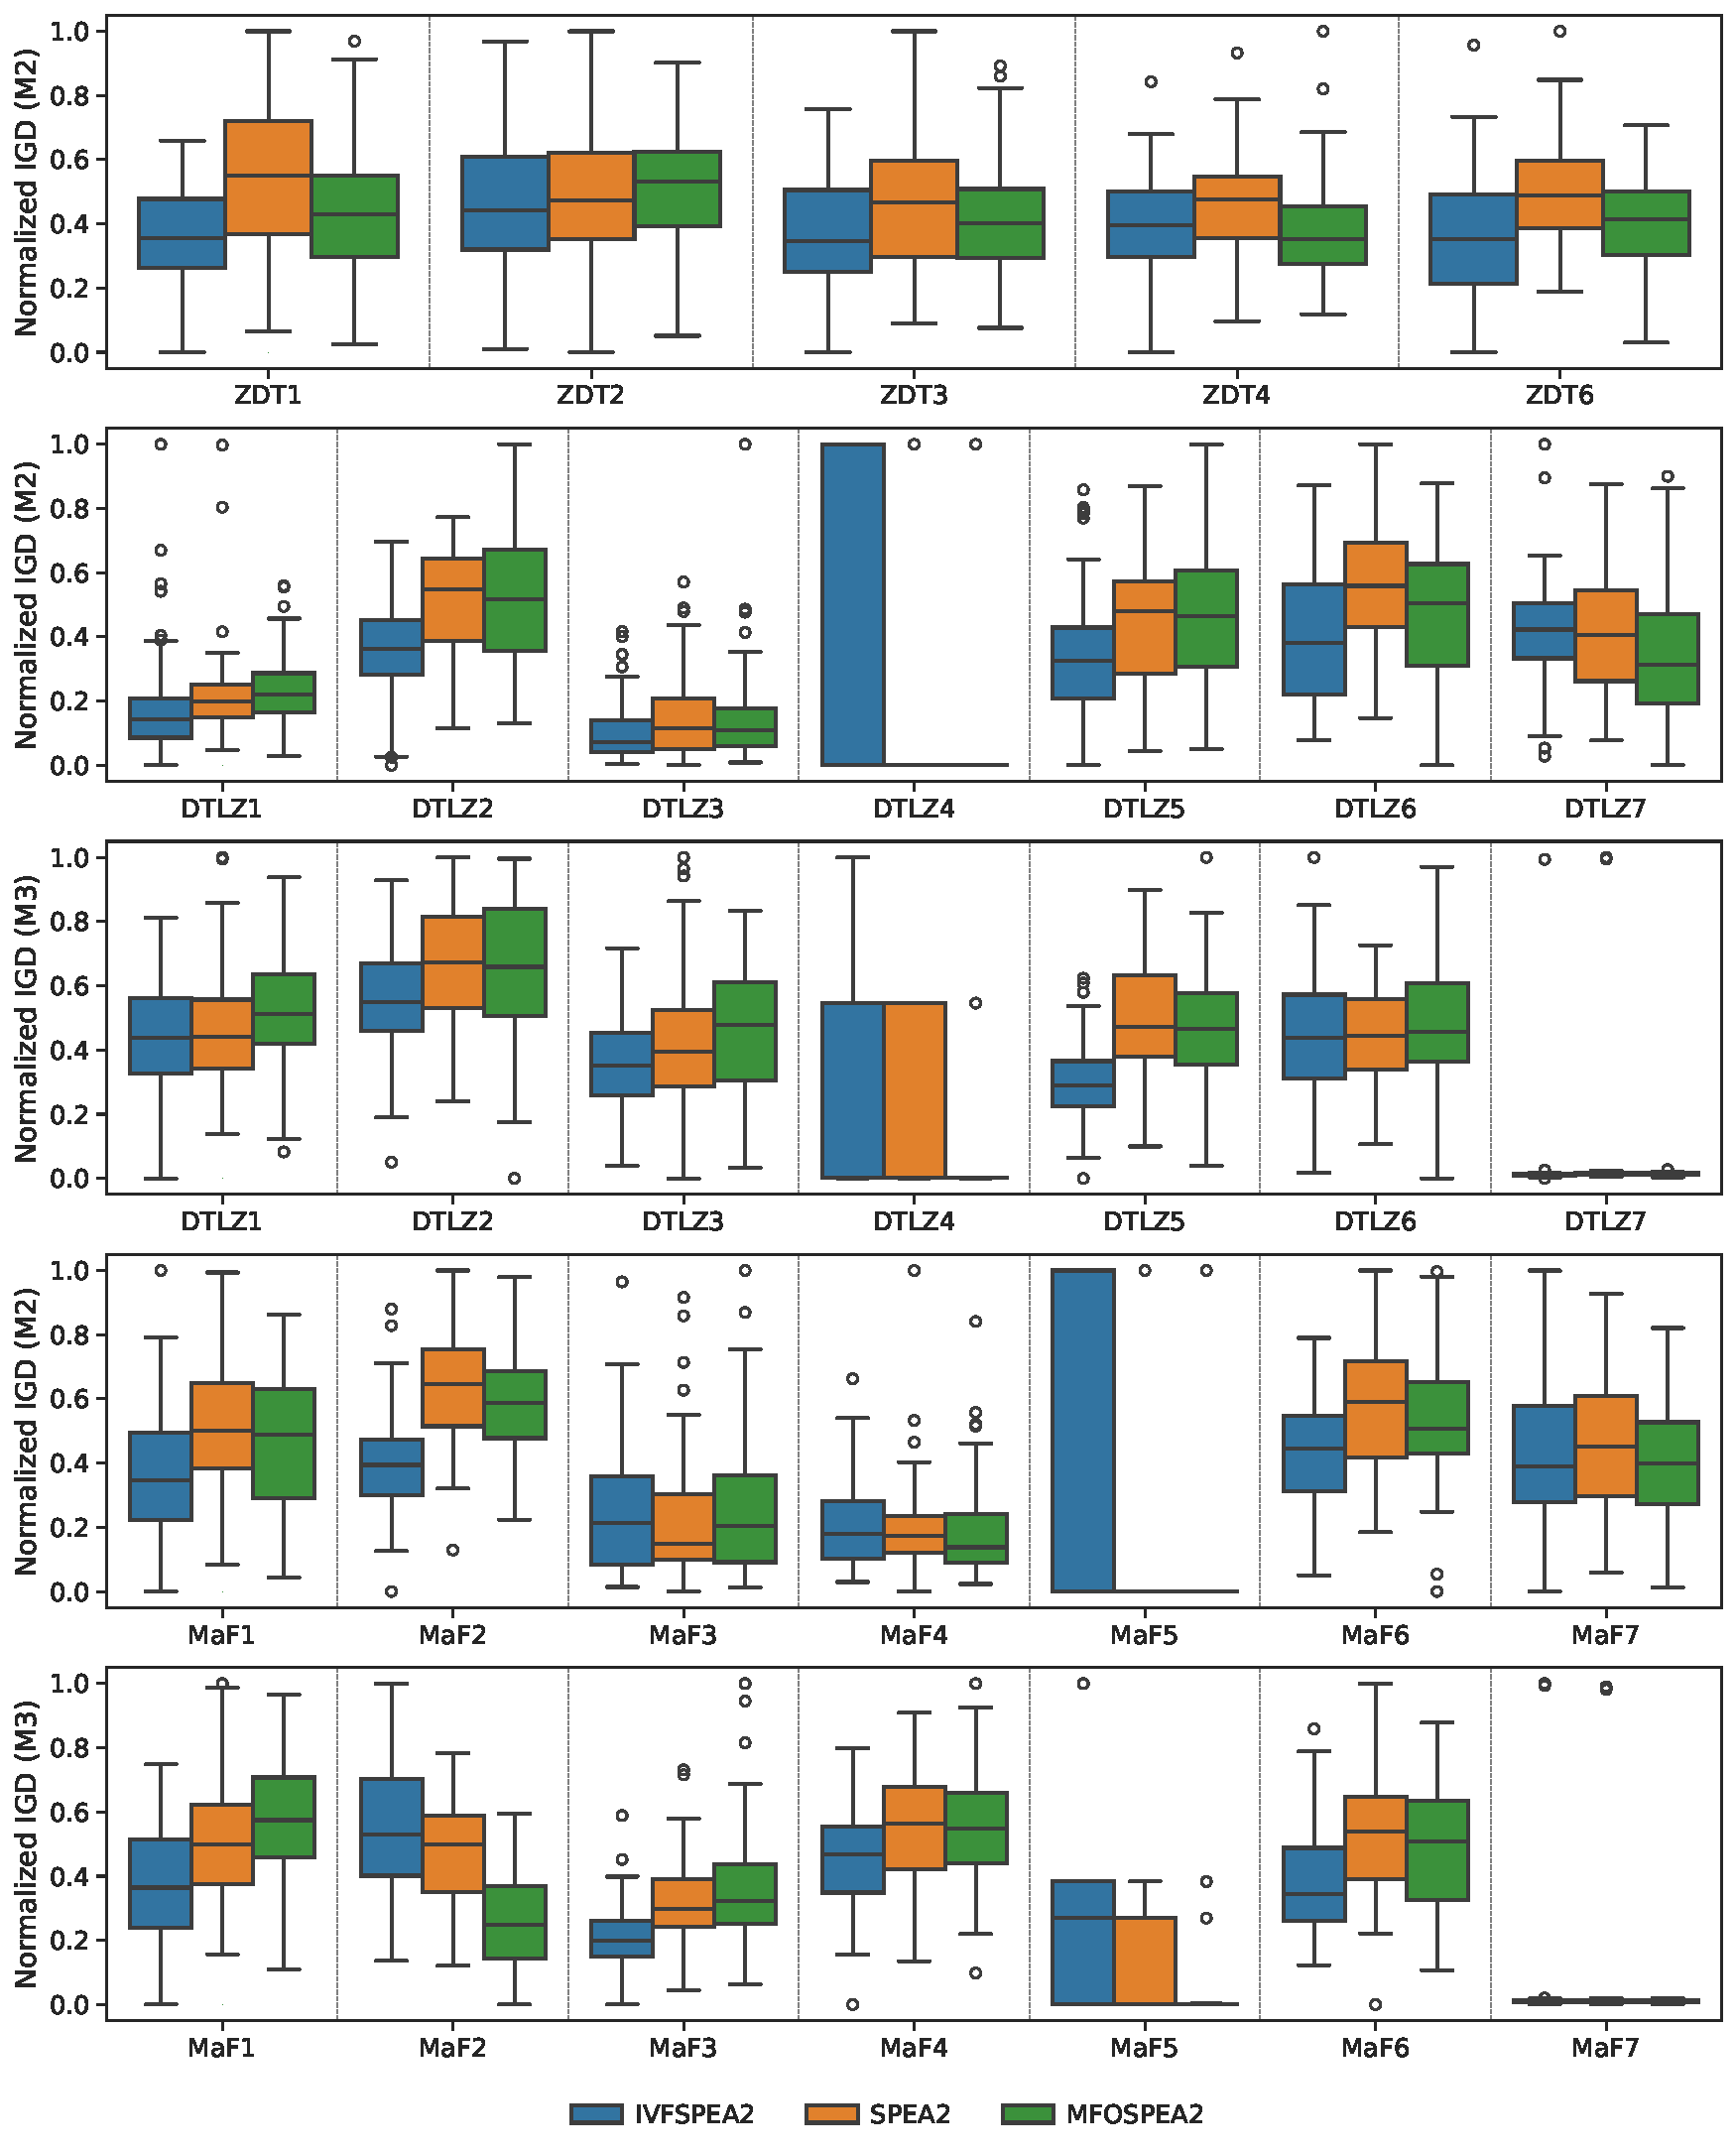
\includegraphics[
    %width=0.95\textwidth,
    height=0.6\textheight]{fig/all_benchmarks_igd_boxplot.pdf}
    \caption{Diagramas de caixa do IGD normalizado para problemas ZDT, DTLZ e MaF (ZDT1-ZDT6, DTLZ1-DTLZ7 e MaF1 - MaF7) com M=2 e M=3 objetivos, comparando IVF/SPEA2, SPEA2 e MFOSPEA2. A linha superior exibe resultados para M=2 objetivos, e a linha inferior para M=3 objetivos para cada problema de referência.}
    \label{fig:all_benchmarks_igd_boxplot}
\end{figure}

A análise abrangente dos problemas de referência revela que o IVF/SPEA2 mantém vantagens consistentes de desempenho através de características diversas de problemas. Na suíte ZDT, o algoritmo demonstra desempenho superior em problemas com frentes de Pareto descontínuas (ZDT3) e paisagens multimodais (ZDT4, ZDT6). Para a família DTLZ, melhorias significativas são observadas particularmente em problemas com frentes de Pareto lineares (DTLZ1, DTLZ2) e geometrias degeneradas (DTLZ5, DTLZ6). Os resultados da suíte MaF confirmam ainda mais a eficácia do algoritmo em problemas multi-objetivo de grande escala e complexos, com ganhos notáveis de desempenho em MaF1, MaF2 e MaF6.

Finalmente, para avaliar a significância prática dessas diferenças de desempenho além de simples comparações de métricas, uma análise estatística rigorosa usando o teste de tamanho de efeito Vargha-Delaney A12 é apresentada. A Figura~\ref{fig:vargha_delaney_comparison_algorithms} exibe os resultados da análise de tamanho de efeito, onde cada célula representa a probabilidade de que o IVF/SPEA2 superará o algoritmo comparado em um dado problema. A análise abrange todos os problemas de referência segregados por dimensionalidade do espaço objetivo, com seis algoritmos competidores: MFOSPEA2, MOEA/D, NSGA-II, NSGA-III, SPEA2 e SPEA2+SDE. A visualização emprega um esquema de codificação por cores para indicar tanto a direção da diferença de desempenho (melhor, igual, pior) quanto a magnitude do tamanho de efeito de acordo com limites estatísticos estabelecidos (negligível, pequeno, médio, grande).

\begin{figure}[!htb]
    \centering
    % Figura para M=2 objetivos (linha superior)
    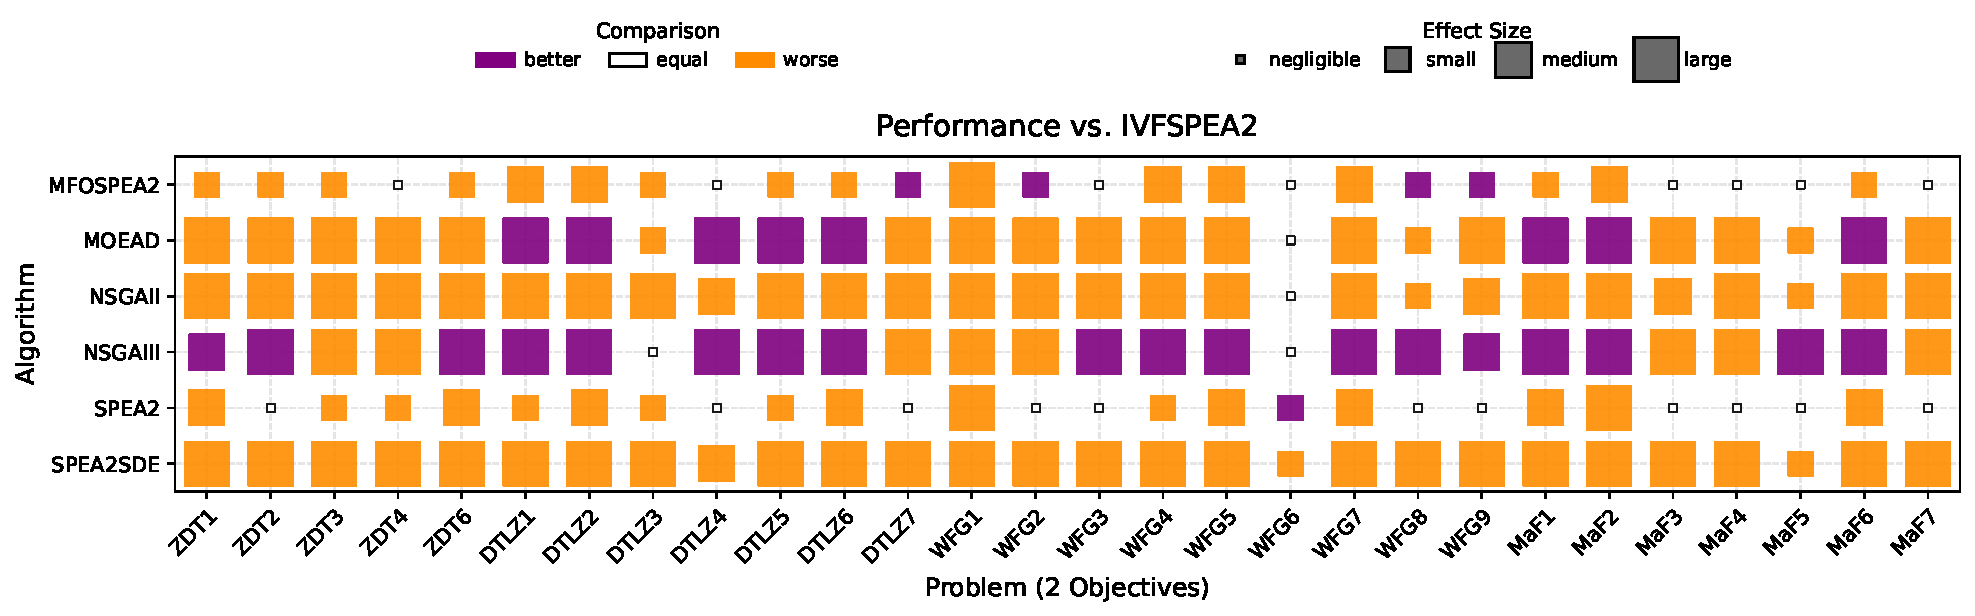
\includegraphics[width=1.0\textwidth]{fig/plot_ZDT_DTLZ_WFG_MaF_M2_Objectives_vs_IVFSPEA2.pdf}
    
    % Espaçamento vertical entre as figuras
    \vspace{0.1cm} 
    
    % Figura para M=3 objetivos (linha inferior)
    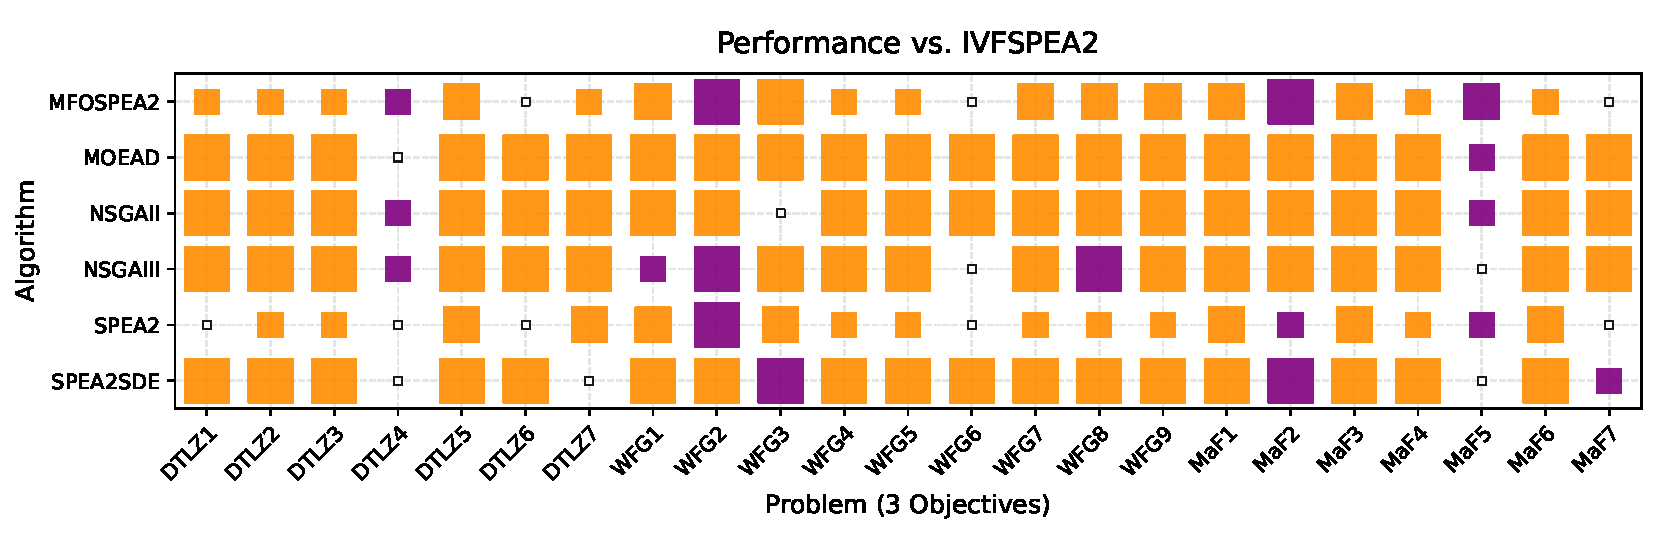
\includegraphics[width=0.85\textwidth]{fig/plot_DTLZ_WFG_MaF_M3_Objectives_vs_IVFSPEA2-b.pdf}
    
    \caption{Análise comparativa de desempenho usando teste de tamanho de efeito Vargha-Delaney para algoritmos de otimização multi-objetivo em problemas de teste de referência. O painel superior mostra resultados para problemas bi-objetivo (M=2): ZDT1-ZDT4, ZDT6, DTLZ1-DTLZ7, WFG1-WFG9 e MaF1-MaF7. O painel inferior apresenta resultados para problemas tri-objetivo (M=3): DTLZ1-DTLZ7, WFG1-WFG9 e MaF1-MaF7. Todos os algoritmos (MFOSPEA2, MOEA/D, NSGA-II, NSGA-III, SPEA2 e SPEA2+SDE) são comparados contra o algoritmo de referência IVF/SPEA2. A codificação por cores indica comparação de desempenho (melhor, igual, pior) e magnitude do tamanho de efeito (negligível, pequeno, médio, grande) de acordo com a estatística A12 de Vargha-Delaney.}
    \label{fig:vargha_delaney_comparison_algorithms}
\end{figure}

A análise de tamanho de efeito fornece evidência do desempenho superior do IVF/SPEA2 com significância estatística. Para problemas bi-objetivo (M=2), o IVF/SPEA2 demonstra vantagens substanciais contra a maioria dos competidores, com tamanhos de efeito predominantemente variando de pequeno a grande através da maioria dos problemas de referência. A dominância de desempenho torna-se ainda mais pronunciada para problemas tri-objetivo (M=3), onde o IVF/SPEA2 exibe superioridade consistente e estatisticamente significativa através dos problemas de referência DTLZ, WFG e MaF contra todos os algoritmos avaliados. Esta análise estatística abrangente reforça que a integração do mecanismo IVF fornece não apenas vantagens mensuráveis mas também praticamente significativas de desempenho através de paisagens diversas de otimização multi-objetivo, estabelecendo a abordagem proposta como um aprimoramento robusto e eficaz para a estrutura SPEA2.
\chapter{Discussão e Conclusões}
\label{sec:discussion_conclusions}

Este estudo investiga o algoritmo híbrido IVF/SPEA2, examinando seu desempenho como um aperfeiçoamento memético para a estrutura SPEA2. Os resultados experimentais indicam que a integração do método de Fertilização In Vitro produz melhorias de desempenho em vários benchmarks de otimização multiobjetivo, embora com graus variados de eficácia dependendo das características do problema.



 A avaliação experimental em 79 instâncias de benchmark revelou que o IVF/SPEA2 mostra desempenho aprimorado em relação ao SPEA2 baseline em muitos casos de teste. Em cenários bi-objetivo (M=2), o algoritmo alcançou superioridade estatística ou equivalência em todas as 28 instâncias de teste, com 16 melhorias significativas (57,1\%) e nenhuma degradação estatisticamente significativa. Para problemas tri-objetivo (M=3), o IVF/SPEA2 obteve 14 vitórias (60,9\%) contra 3 derrotas (13,0\%). Embora esses resultados sugiram benefícios potenciais, as melhorias são observadas principalmente em estruturas específicas de problemas, em vez de uniformemente em todos os tipos de benchmark.

 Quando comparado a outros algoritmos estabelecidos (NSGA-II, NSGA-III, MOEA/D, MFOSPEA2, SPEA2+SDE), o IVF/SPEA2 demonstra desempenho competitivo. O algoritmo mostra algumas vantagens sobre o NSGA-III, particularmente em cenários tri-objetivo onde o desempenho do NSGA-III parece declinar. No entanto, as vantagens comparativas são modestas e dependentes do problema, sugerindo que nenhum algoritmo único domina todos os tipos de problema.

 A análise do tamanho do efeito Vargha-Delaney $A_{12}$ indica diferenças práticas além da significância estatística em certos casos. O algoritmo demonstra tamanhos de efeito variados entre as categorias de benchmark, com desempenho mais forte em problemas apresentando geometrias regulares de frente de Pareto (MaF1, MaF3, MaF6: $A_{12} > 0,71$).

A análise sugere que as características de desempenho do IVF/SPEA2 derivam de vários fatores:

A análise sugere que as características de desempenho do IVF/SPEA2 derivam de vários fatores, como por exemplo as operações de cruzamento direcionadas do mecanismo IVF podem ajudar a abordar a estagnação evolutiva em certos cenários. A intervenção estratégica (c=10\%, r=10\%) parece manter alguma pressão evolutiva enquanto potencialmente previne a estagnação populacional em tipos específicos de problemas. No entanto, a eficácia varia consideravelmente entre diferentes paisagens de otimização.

 O algoritmo mostra eficácia particular em problemas com certas características estruturais, como frentes de Pareto lineares, convexas ou degeneradas (DTLZ1, DTLZ2, DTLZ5, DTLZ6). Inversamente, a abordagem enfrenta limitações em paisagens altamente enganosas (MaF2, WFG2), onde os mecanismos elitistas combinados podem levar à convergência prematura. Este desempenho dependente do problema sugere que a abordagem não é universalmente benéfica.

A estrutura de análise estatística, incorporando testes de soma de postos de Wilcoxon e medições de tamanho de efeito Vargha-Delaney, fornece evidências para diferenças de desempenho em casos específicos. No entanto, a significância prática dessas melhorias deve ser avaliada dentro do contexto de requisitos específicos de aplicação e restrições computacionais.

 A integração de mecanismos IVF no SPEA2 demonstra uma possível abordagem para aperfeiçoamento memético de estruturas evolutivas estabelecidas. Embora mostre promessa em certos cenários, os benefícios da abordagem parecem limitados a características específicas de problemas, em vez de fornecer melhorias universais.

 A análise revela relações entre mecanismos algorítmicos e características estruturais do problema. A identificação de tipos de problemas favoráveis (geometrias regulares de Pareto) e casos desafiadores (paisagens altamente enganosas) fornece insights para seleção de algoritmos, embora seja necessária validação mais extensa.

 Problemas com múltiplos objetivos conflitantes apresentando estruturas regulares de trade-off podem se beneficiar desta abordagem, embora análise cuidadosa do problema seja necessária para determinar adequação.

 Aplicações onde as características do problema se alinham com as forças demonstradas do algoritmo poderiam potencialmente se beneficiar desta abordagem híbrida.

A investigação experimental sugere que o IVF/SPEA2 representa um aperfeiçoamento modesto ao SPEA2 para certos tipos de problemas. A integração do mecanismo de Fertilização In Vitro mostra benefícios potenciais em contextos específicos, embora as melhorias não sejam nem universais nem dramáticas. O desempenho do algoritmo é notavelmente dependente da estrutura do problema, limitando sua aplicabilidade geral.

A pesquisa fornece alguma evidência para o potencial de aperfeiçoamentos meméticos direcionados em otimização evolutiva multiobjetivo. No entanto, a natureza específica do problema das melhorias destaca a importância da seleção cuidadosa de algoritmos baseada em características do problema, em vez de assumir superioridade universal.
s.
\chapter{Ameaças à Validade}
\label{sec:threats}

Embora os resultados experimentais demonstrem a eficácia do algoritmo IVF/SPEA2 em vários problemas de benchmark, diversas ameaças à validade devem ser reconhecidas para fornecer uma avaliação abrangente das limitações e da generalização do estudo. O estudo esforçou-se para abordar essas ameaças por meio de seu desenho e escolhas analíticas.

\section{Validade Interna}

\textbf{Viés de Configuração de Parâmetros:} Os parâmetros do método IVF (Tamanho da Coleta $c=10\%$ e Taxa $r=10\%$), embora configurados com base em investigações preliminares e para consistência com trabalhos relacionados anteriores para fornecer uma linha de base fundamentada, não foram otimizados para cada classe de problema específica. Esta abordagem visou demonstrar o impacto geral do método IVF com um conjunto de parâmetros consistente e comum, onde o artigo observa que um ``envolvimento relativamente modesto do método IVF'' com esses parâmetros foi frequentemente suficiente para produzir melhorias estatisticamente significativas.

\textbf{Viés de Seleção de Benchmark:} Embora o estudo tenha utilizado conjuntos de benchmarks bem estabelecidos (ZDT, DTLZ, WFG e MaF) selecionados por suas ``características complementares e níveis de complexidade variados'' e capacidade de cobrir uma ``ampla gama de geometrias da fronteira de Pareto e complexidades de problemas'' (incluindo frentes convexas, côncavas, desconectadas, não separáveis, multimodais e assimétricas), a eficácia do algoritmo ainda pode ser dependente do problema. Isso é sugerido pelo desempenho variado em problemas específicos, como MaF2 e WFG2, que em alguns cenários tri-objetivo apresentaram resultados estatisticamente inferiores para o IVF/SPEA2. A seleção diversificada, no entanto, visou fornecer um ambiente de teste desafiador para avaliar a versatilidade.

\textbf{Variabilidade da Implementação:} A implementação do IVF/SPEA2 na estrutura PlatEMO, uma reconhecida ``plataforma MATLAB para otimização multiobjetivo evolutiva'', ajuda a garantir a reprodutibilidade e reduzir a variabilidade em comparação com uma implementação totalmente personalizada. Embora escolhas específicas para operadores (por exemplo, tipos AR e EAR para IVF) e outros detalhes específicos da estrutura possam influenciar os resultados, o uso de uma plataforma padrão mitiga essa preocupação.

\textbf{Natureza Estocástica dos Algoritmos:} Para levar em conta a estocasticidade inerente dos algoritmos evolutivos, tanto o IVF/SPEA2 quanto o SPEA2 foram executados ``100 vezes, coletando desempenho na métrica IGD'' para cada configuração de teste. A significância estatística das diferenças foi então avaliada usando o teste de soma de postos de Wilcoxon, que é apropriado para comparar distribuições de múltiplas execuções.

\section{Validade Externa}


\textbf{Limitação de Benchmarks Sintéticos:} Todos os problemas testados são benchmarks sintéticos (ZDT, DTLZ, WFG e MaF). Embora estes sejam ``amplamente reconhecidos'' e projetados para exibir propriedades matemáticas específicas que testam diversas capacidades algorítmicas (como ``não separabilidade, multimodalidade, assimetria'' para WFG ou geometrias variadas da fronteira de Pareto para ZDT e DTLZ), seu desempenho pode não se traduzir diretamente para problemas de otimização do mundo real com complexidades adicionais. No entanto, este ambiente controlado é padrão para avaliação rigorosa, e o artigo observa que o SPEA2 foi aplicado com sucesso em diversos campos, sugerindo potencial para sua versão aprimorada.

\textbf{Configuração Experimental Fixa:} O estudo empregou tamanhos de população fixos ($N=100$) e um número definido de avaliações de função ($FE=100.000$) em todos os problemas e algoritmos. Essa consistência garante uma base justa para comparação e se alinha com as práticas comuns na literatura, embora essas configurações específicas possam não ser ótimas para a complexidade ou dimensionalidade de cada problema individual.

\section{Validade de Construto}

\textbf{Limitações da Métrica de Desempenho:} O estudo baseia-se na métrica de Distância Geracional Invertida (IGD), que é um ``indicador de desempenho amplamente adotado'' que mede tanto a convergência quanto a diversidade. Para fornecer uma perspectiva mais nuançada além do IGD e dos valores-p, o estudo também incorporou a análise de tamanho de efeito A12 de Vargha-Delaney, oferecendo insights sobre a ``probabilidade de que uma solução selecionada aleatoriamente do IVF/SPEA2 supere uma solução selecionada aleatoriamente do algoritmo de comparação''.

\textbf{Suposições do Teste Estatístico:} O teste de soma de postos de Wilcoxon, ``um teste de hipótese estatístico não paramétrico'', foi usado para avaliar a significância estatística. Essa escolha é robusta, pois ``não faz suposições sobre a normalidade das distribuições dos dados'', tornando-o adequado para comparar algoritmos evolutivos. Além disso, a realização de 100 execuções independentes para cada configuração fortalece a confiabilidade das conclusões estatísticas.

\section{Validade da Conclusão}

\textbf{Generalização Além do Algoritmo Hospedeiro:} O mecanismo IVF foi testado exclusivamente dentro da estrutura SPEA2 neste estudo específico, pois essa hibridização é a proposta central. Embora os benefícios observados estejam diretamente ligados a essa combinação, o artigo também referencia integrações bem-sucedidas anteriores do método IVF com outros algoritmos como NSGA-II e GDE3, sugerindo que o próprio método IVF tem potencial como um módulo auxiliar de aplicação mais geral.

Essas ameaças à validade identificadas fornecem contexto para a interpretação dos resultados e destacam áreas onde pesquisas futuras, conforme delineado na Seção \ref{sec:future_work}, poderiam fortalecer ainda mais as evidências para a abordagem IVF/SPEA2.
\chapter{Trabalhos Futuros}
\label{sec:future_work}

Com base nos resultados, conclusões e ameaças à validade identificadas neste estudo, delineamos várias direções promissoras para pesquisas futuras que abordam as limitações identificadas e expandem o escopo da investigação:

\section{Aprimoramentos Metodológicos}

\begin{enumerate}
\item \textbf{Otimização e Adaptação de Parâmetros:} Desenvolver estratégias para configuração automática dos parâmetros do IVF (Tamanho da Coleta $c$ e Taxa $r$), superando o viés de configuração identificado na Seção~\ref{sec:threats}. Isso inclui:
\begin{itemize}
\item Investigação de técnicas de meta-otimização para encontrar configurações ótimas específicas para cada classe de problema;
\item Desenvolvimento de mecanismos adaptativos que ajustem dinamicamente os parâmetros durante a evolução com base em métricas de diversidade populacional e convergência;
\end{itemize}

\item \textbf{Integração com Outros Algoritmos Base:} Expandir a investigação do mecanismo IVF além do SPEA2, incorporando-o sistematicamente em outros algoritmos evolutivos multiobjetivo estabelecidos (NSGA-III, MOEA/D-variants, SMS-EMOA) para avaliar sua generalidade como módulo auxiliar.
\end{enumerate}

\section{Validação Experimental Abrangente}

\begin{enumerate}
\item \textbf{Avaliação em Problemas do Mundo Real:} Abordar a limitação de benchmarks sintéticos através da aplicação sistemática do IVF/SPEA2 em problemas de otimização do mundo real de diferentes domínios, entendendo por exemplo o impacto nos exemplos reais onde o SPEA2 vem sendo aplicado.



\item \textbf{Estudos de Escalabilidade:} Investigar o comportamento do algoritmo com diferentes tamanhos de população e orçamentos computacionais, superando a limitação de configuração experimental fixa identificada nas ameaças à validade.
\end{enumerate}

\section{Extensões Algorítmicas}

\begin{enumerate}
\item \textbf{Variantes Híbridas Avançadas:} Explorar combinações do mecanismo IVF com outras técnicas de aprimoramento, como:
\begin{itemize}
\item Busca local multiobjetivo;
\item Técnicas de niching e clustering;
\item Abordagens baseadas em aprendizado de máquina para guiar a seleção.
\end{itemize}

\item \textbf{Paralelização e Computação Distribuída:} Desenvolver versões paralelas e distribuídas do IVF/SPEA2 para lidar com problemas computacionalmente intensivos e aproveitar arquiteturas de computação modernas.

\item \textbf{Integração com Técnicas de Surrogate Modeling:} Investigar a combinação do IVF/SPEA2 com modelos substitutos para problemas com avaliações de função computacionalmente caras.
\end{enumerate}

Estas direções de pesquisa futura abordam sistematicamente as limitações identificadas nas ameaças à validade e proporcionam uma base sólida para o avanço contínuo da área de otimização evolutiva multiobjetivo, contribuindo tanto para o desenvolvimento teórico quanto para aplicações práticas relevantes.

%------------------------------------------------------------ BIBLIOGRAFIA %
\cleardoublepage
% \nocite{*} % Ative somente quando for necessário listar referências não citadas.
\arial
\bibliography{./bib/modelo-tese} %%% Nomes dos seus arquivos .bib
\label{ref-bib}

%--------------------------------------------------------------- APÊNDICES %
% \apendices

% \input{./pos/apend_I}
% \input{./pos/apend_II}

\end{document}

%------------------------------------------------------------------------- %
%        F I M   D O  A R Q U I V O :  m o d e l o - t e s e . t e x       %
%------------------------------------------------------------------------- %
